\documentclass[14pt,a4paper,onecolumn]{extarticle}
\usepackage[utf8]{inputenc}
\usepackage{amsmath}
\usepackage{amsfonts}
\usepackage{amssymb}
\usepackage{graphicx}
\usepackage{natbib}
\usepackage{multirow}
\usepackage{pdflscape}

\bibliographystyle{plainnat}
\setlength{\parskip}{1.2em}
\setlength{\parindent}{0pt}
% \graphicspath{{../../images/}}

\author{Ibrahim AbuBakr ElSeddiq}
\title{The predictive value of NTproBNP on postoperative outcome in patients undergoing offpump CABG}

\begin{document}

\maketitle
\clearpage
\clearpage
\section{Review of Literature}

\subsection{Natriuretic Peptides}


The history of the NP class of biomarkers dates back to 1950s when early electron microscopy studies reported dense granules in the atrial myocardium similar to glandular tissue from endocrine organs. Soon, the close interplay between atria and intravascular volume was revealed; stretching of canine left atrium increased urine output and injection of atrial tissue into rats caused diuresis and natriuresis. Atrial natriuretic peptide (ANP) was subsequently purified, sequenced, and reproduced. \citep{Gaggin2014}

Subsequent studies were aimed at discovering family members which resulted in the isolation of two other factors which were named brain natriuretic peptide (BNP) and C-type natriuretic peptide (CNP). Studies also showed that although BNP was first isolated from the brain, that it is predominantly expressed in the ventricle. ANP and BNP were therefore renamed A-type and B-type natriuretic peptide, respectively, to better reflect their position in the family and to also lessen the misleading nature of the nomenclature of BNP as a cardiovascular and not a neural factor. ANP and BNP are the natriuretic peptides which are expressed predominantly in the atria and ventricle, respectively, and are referred to as the cardiac natriuretic peptides. CNP is differentially expressed mainly in the nervous system and vasculature (e.g. endothelial cells, monocyte / macrophages) and is involved mainly in neural regulation as well as vascular control although its role is still unclear. \citep{Suzuki2001}

Other NPs that share a common biochemical structural feature, a 17-amino-acid ring and a disulfide bridge between cysteine molecules, have been discovered since: urodilantin (an isoform of ANP), C-type natriuretic peptide, and Dendroaspis natriuretic peptide. \citep{Gaggin2014}

Each natriuretic peptide is coded by a separate gene but shows similar exon–intron properties. In humans, the ANP and
BNP genes are located 8 kilobases apart on chromosome 1
and the CNP gene is located on chromosome 2. Each natriuretic peptide gene produces a prohormone or precursor protein. ANP is synthesized as a 126 amino acid precursor protein which is cleaved to produce a 96 amino acid amino-terminal fragment and a 28 amino acid carboxyl-terminal fragment. The carboxyl-terminal 28 amino acid fragment is the biologically active peptide and has a shorter half-life than the amino-terminal fragment. Similarly, BNP is produced as a 108 amino acid precursor protein which is cleaved into a biologically active 32 amino acid carboxyl-terminal fragment and a 76 amino acid amino-terminal fragment. CNP produces 22 and 53 amino acid fragments. The 22 amino acid fragment is the mature and more active form, and is expressed in the nervous system and endothelial cells. The common property of the natriuretic peptides is the formation of a disulfide bond which results in a ringed structure (Fig. 1).\citep{Suzuki2001}




ANP is encoded by the NPAA gene on chromosome 1. It is translated into a 151-amino-acid pre-prohormone (preproANP) that is cleaved in the sarcoplasmic reticulum to a 126-amino-acid prohormone (proANP), which is stored in intracellular granules.  When stimulated and released, proANP is further cleaved into a 28-amino-acid bioactive form (ANP) and a 98-amino-acid N-terminal fragment (NT-proANP). The half-life of ANP is approximately 2 minutes, whereas NT-proANP half-life is variable depending on the fragment measured. \citep{Maisel2018}



The biological actions of natriuretic peptides are mediated through membrane-bound natriuretic peptide receptors (NPR) that are linked to a cyclic guanosine monophosphate-dependent signaling cascade, including NPR-A, which preferentially binds ANP and BNP, and NPR-B, which preferentially binds CNP.

Elevated natriuretic peptides levels can be found in many circumstances involving LV dysfunction or hypertrophy; right ventricular (RV) dysfunction secondary to pulmonary diseases; cardiac inflammatory or infectious diseases; and endocrinologic diseases and high output status without decreased left ventricular ejection fraction (EF), e.g., sepsis, renal failure, cirrhosis of liver, or intracranial pathologies. The causes and mechanisms of elevated natiuretic peptides levels are summarized in Fig. \ref{NP_causes}. %The potential clinical applications in the non-HF settings are summarized in Table \ref{NP_applications}.

\begin{figure}
    \centering
    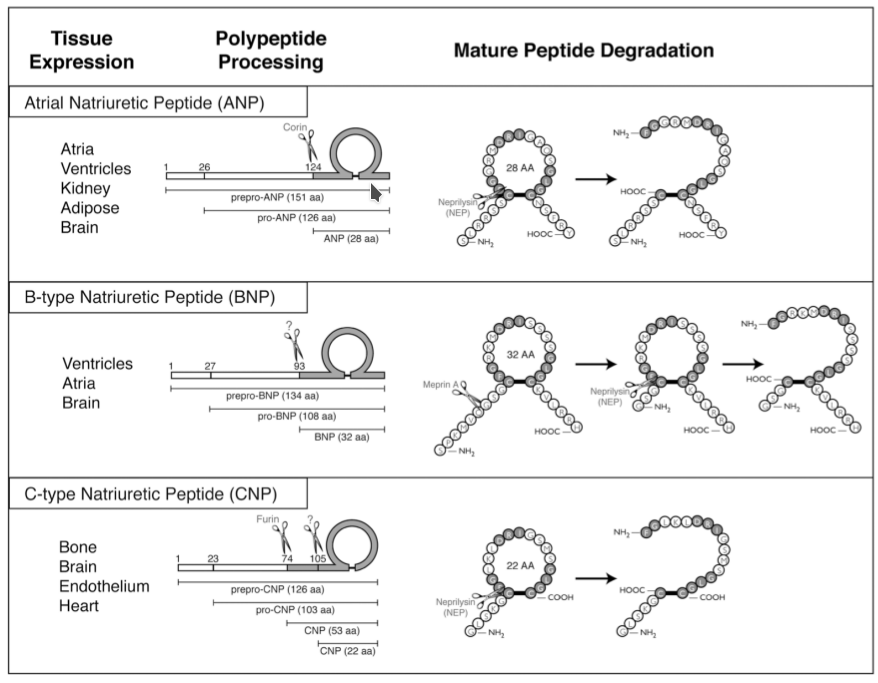
\includegraphics[scale=0.4]{../../images/NP_structure.png}
    \caption{Structure of the human natriuretic peptides. The structure of the preprohormones for ANP, BNP and CNP are outlined on the left of each panel. The final amino acid sequence and structure of the mature peptides along with the major degradation product are shown on the right. The sites of cleavage are indicated with scissors.}
    \label{NP_structure}
\end{figure}

\subsubsection{Atrial Natriuretic Peptide}

All natriuretic peptides are synthesized as preprohormones Fig \ref{NP_structure}.
The resulting mRNA gives rise to a 151 amino acid polypeptide, known as preproANP. The first 25 amino acids constitute a signal sequence that is cleaved to yield a 126 amino acid peptide called proANP, which is the major form of ANP stored in the atrial granules \citep{Oikawa1984}.
Upon release from these granules, proANP is rapidly cleaved by corin, a transmembrane cardiac serine protease. Corin is highly expressed on the extracellular surface of atrial cardiomyocytes and cleaves proANP into the biologically active 28-amino acid form of ANP \citep{Yan2000}.
%Mice lacking functional corin have dramatically reduced levels of fully processed ANP in their hearts and are mildly hypertensive \citep{Chan2005}.
Alternative processing of proANP in the kidney by an unknown protease results in a 32-amino acid peptide called urodilatin that contains four additional amino-terminal residues \citep{Forssmann1998}.
% Disruption of the murine ANP gene, results in marked hypertension, which was initially described as salt-sensitive \citep{John1995}, but later found not to be correlated with dietary salt intake \citep{John1996}.

Release of proANP from the atrial granules is primarily stimulated by stretch of the atrial wall caused by increased intravascular volume \citep{Bilder1986} \citep{Edwards1988} \citep{Lang1985}, but pressor hormones also stimulate ANP release \citep{Ruskoaho2003}.
%Upon secretion and cleavage into the mature peptide, ANP enters the coronary sinus and is distributed to its target organs via the circulation.
Plasma levels of ANP are relatively low (10 fmol/ml), but in patients with congestive heart failure, circulating ANP levels are elevated from 10- to 30-fold \citep{Burnett1986} \citep{Cody1986}.

% The plasma half-life of ANP in humans is approximately 2 min \citep{Nakao1986} \citep{Yandle1986}. Degradation of the active ANP peptide occurs through the actions of neutral endopeptidase (NEP) \citep{Stephenson1987} \citep{Vanneste1988} as well as through binding to the natriuretic peptide clearance receptor (NPR-C), a cell surface receptor that lacks guanylyl cyclase activity and controls the local concentrations of natriuretic peptides via constitutive receptor mediated internalization and degradation. Inhibiting NEP, increases the half-life of ANP \citep{Yandle1989}, suggesting that NEP activity contributes to the rapid clearance of ANP. However, it is important to note that mice lacking functional NEP do not exhibit increased natriuretic peptide function \citep{Lu1995}. In contrast, mice lacking NPR-C are hypotensive, exhibit skeletal overgrowth and have reduced ability to clear ANP compared to wild type mice, suggesting that NPR-C is also a physiologic regulator of circulating natriuretic peptide concentrations \citep{Matsukawa1999}.

ANP is secreted in response to:
    \begin{itemize}
        \item Stretching of the atrial wall \citep{Widmaier2008}
        \item Reduced Sympathetic stimulation of $\beta$-adrenoceptors
        \item Raised sodium concentration (hypernatremia), though sodium concentration is not the direct stimulus for increased ANP secretion. \citep{Widmaier2008}
        \item Endothelin, a potent vasoconstrictor
        \item exercise \citep{Kokkonen2002}
    \end{itemize}


\begin{figure}
    \centering
    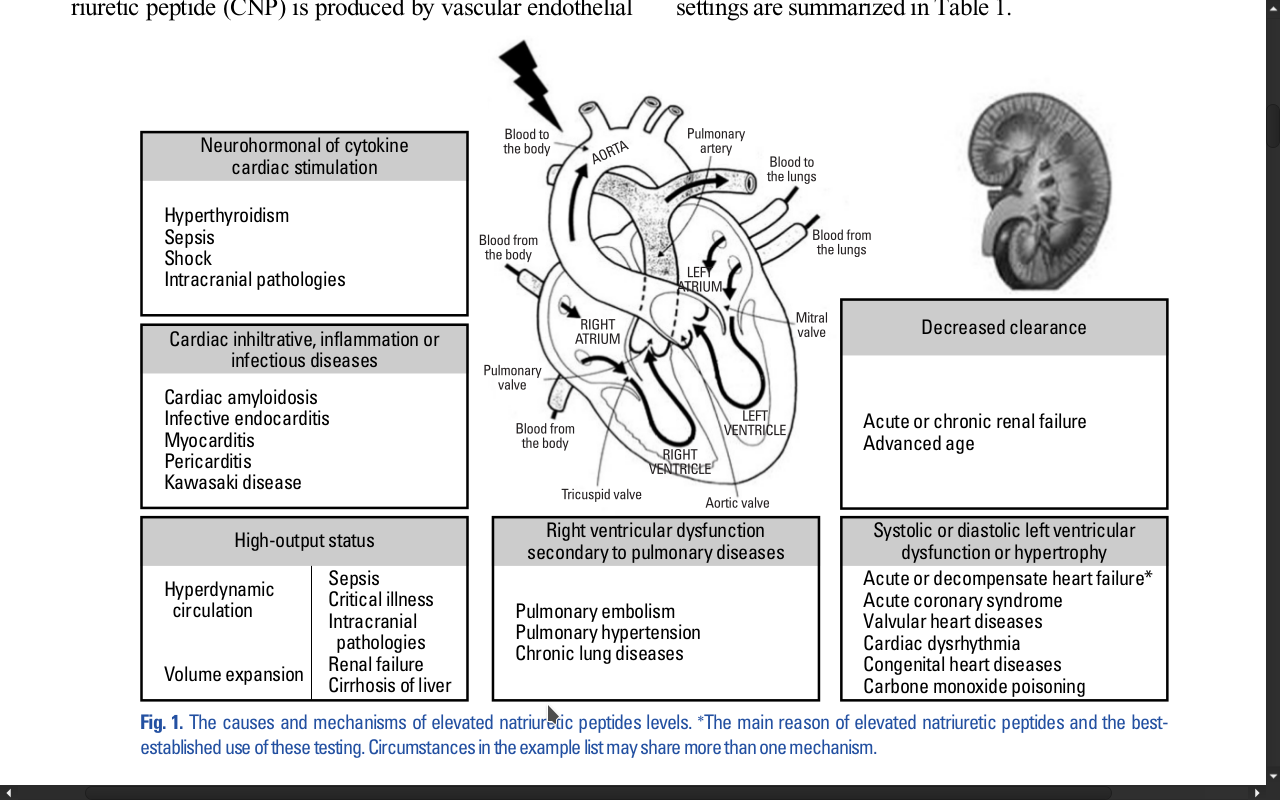
\includegraphics[scale=0.3]{../../images/NP_causes.png}
    \small\caption{The causes and mechanisms of elevated natriuretic peptides levels.}
    \label{NP_causes}
\end{figure}

% \begin{table}
%     \centering
%     \caption{Potential Clinical Applications of Natriuretic Peptides in Selected Diseases}
%     \begin{tabular}{|l|c|c|c|}
%         \hline
%         Diseases & Screening \footnote{Screening for the presence of cardiac dysfunction} &  & Prognosis \\
%         \hline
%         Heart failure \footnote{The best-established clinical application of these natriuretic peptides testing} & + & + & + \\
%         Acute coronary syndrome & + & + & + \\
%         Cardiac procedures & + & + & + \\
%         Pulmonary embolism & + & + & + \\
%         Pulmonary hypertension & + & + & - \\
%         Chronic lung diseases & + & + & + \\
%         Valvular heart diseases & + & + & N/A \\
%         Cardiac dysrhythmia & + & + & +/- \\
%         Cardiac inflammatory or infectious diseases & + & + & N/A \\
%         Cardiogenic syncope & + & N/A & N/A \\
%         Sleep apnea & + & + & N/A \\
%         Hypertension & + & + & N/A \\
%         Sepsis & + & + & + \\
%         Renal failure & + & + & + \\
%         Cirrhosis of liver & + & + & + \\
%         Hyperthyroidism & + & + & N/A \\
%         Intracranial pathologies & + & + & + \\
%         Epilepsy / Seizures & + & - & - \\
%         Carbone monoxide poisoning & + & N/A & N/A \\
%         \hline
%     \end{tabular}
%     \label{NP_applications}
% \end{table}

\subsubsection{B-Type Natriuretic Peptide}
BNP was initially purified and sequenced from extracts of porcine brain tissue and hence it was named brain natriuretic peptide \citep{Sudoh1988}. Subsequently, BNP was found at much higher concentrations in cardiac tissues \citep{Mukoyama1991} \citep{Mukoyama1990}.

%PreproBNP is 134 amino acids in length, consisting of a 26 amino acid signal sequence followed by 108 amino acids that constitute proBNP. Unlike preproANP, which has high species homology throughout the entire polypeptide sequence, preproBNP sequences in mammals only have high homology at the amino and carboxyl terminal ends of the polypeptide. For example, the homology of canine preproBNP to human preproBNP is 53\%, whereas the homology for preproANP between these species is 85\%. This lower level of homology gives rise to differing lengths of the active, circulating BNP between mammalian species. For example, in humans and pigs circulating BNP is 32 amino acids in length, while in rats and mice the circulating form is 45 amino acids. The peptidase that cleaves proBNP to its active form has not been identified, but corin is a reasonable suspect.

Although low levels of BNP are stored with ANP in atrial granules, BNP is found at greater concentrations in cardiac ventricles. In this tissue, BNP is not stored in granules, but rather transcribed as needed in response to cardiac stress states. \citep{Grepin1994} \citep{Thuerauf1994} In normal human subjects, plasma concentrations of BNP are very low (1 fmol/ml), but in response to congestive heart failure, circulating concentrations of BNP are dramatically elevated \citep{Mukoyama1991} \citep{Mukoyama1990}.

BNP can be produced in both atria and ventricles, and is upregulated in failing ventricular myocardium. In response to increased myocardial stretch and wall stress, ventricular myocytes secret the pro-hormone pre-proBNP, which is then cleaved into biologically active BNP and the inactive byproduct N-terminal-proBNP (NT-proBNP). Elevated BNP levels have been demonstrated to be a response to increased angiotensin II and sympathetic tones. \citep{Iwanaga2006}


BNP is eliminated by binding to the NPR-C or degradation by NEP on endothelial cells, smooth muscle cells, cardiac myocytes, renal epithelium, and fibroblasts. NT-proBNP is cleared mainly by the kidney.\citep{Schrier1999}  Compared to ANP, circulating BNP has a significantly longer half-life of around 20 min in humans \citep{Mukoyama1991} \citep{Mukoyama1990}; the half-life of NT-proBNP is about 60-90 minutes and would be expected to be longer in the setting of renal dysfunction. Unlike ANP, BNP is not initially cleaved by NEP. Instead, the first six amino-terminal amino acids of BNP are first cleaved by the metalloprotease, meprin A in the kidney brush border, which then allows further degradation by NEP \citep{Pankow2007}. Obese patients tend to have lower BNP levels than others. Neural endopeptidases that can be secreted by adipose tissue may be related to increased BNP clearance in obese patients.\citep{Yang2004}

% todo find the missing citations
Plastic tubes containing ethylenedinitrolotetraacetic acid (EDTA) are desirable for BNP determination and refrigeration is required if the interval between blood collection and analysis is over 4 hours; whereas NT-proBNP can be measured in both serum or plasma, collected in glass or plastic tubes, and has no significant loss of immunoreactivity after 48 hours at room temperature. \citep{Omland2008}
 % A multicenter colloborative proficiency testing study conducted in 90 Italian laboratories had demonstrates that there are significant differences in analytical characteristics and measured values among the most popular commercial methods for BNP and NT-proBNP. Thus, clinicians should be very careful when comparing results obtained by laboratories that use different methods.
 %\citep{Prontera2009}

%Both knockout and overexpression models of NPPB have been generated in mice. The knockout model of Nppb was created by targeted deletion of exons 1 and 2 \citep{Tamura2000}. In contrast to ANP knockout mice, Nppb -/- mice showed no signs of systemic hypertension or ventricular hypertrophy on standard or high salt diets. However, Nppb -/- mice had ventricular fibrotic lesions that increased in size and number in response to pressure overload, compared to wild type animals. Thus, these studies suggest that BNP is not a regulator of blood pressure, at least in mice. Rather, it is a paracrine regulator of cardiac remodeling. In murine overexpression models of BNP, blood pressure reduction of 20 mmHg was seen with 10- to 100-fold increases in plasma BNP levels \citep{Ogawa1994a}. Interestingly, these mice had marked increases in long bone length compared to their wild-type littermates, which most likely resulted from overactivation of NPR-B, the receptor of CNP

\subsubsection{C-Type Natriuretic Peptide}
C-type natriuretic peptide (CNP) was initially purified and sequenced from porcine brain extracts \citep{Sudoh1990}. It is the most highly expressed natriuretic peptide in the brain but is also highly expressed in chondrocytes and endothelial cells. Unlike ANP and BNP, the human gene encoding CNP, NPPC, is not located on chromosome 1 but on chromosome 2 \citep{Ogawa1994b}.

%NPPC encodes a polypeptide of 126 amino acids, with a 23 amino acid signal sequence followed by a 103 amino acid proCNP \citep{Tawaragi1991}. PreproCNP shows remarkable homology between species, even more so than preproANP. The preproCNP polypeptides of mammalian species show 99, 96, 91, and 94\% homology to the human form in chimpanzees, dogs, mice, and rats, respectively. Perhaps even more telling is that the circulating 22 amino acid carboxyl terminal form of CNP is absolutely identical in all of the above species.

Processing of proCNP to its mature form may occur through the action of the intracellular serine endoprotease, furin. In vitro, furin cleaves the 103 amino acid proCNP into a 53 amino acid carboxyl-terminal biologically active peptide \citep{Wu2003a}. This 53 amino acid form of CNP (CNP-53) is the major active form of CNP, at the tissue level \citep{Brown1997}. However, in the systemic circulation, a shorter 22 amino acid form dominates (CNP-22). The protease responsible for this cleavage is not known. Importantly, CNP-53 and CNP-22 appear to bind and activate their cognate receptor, NPR-B, equally well \citep{Yeung1996}.

CNP is not stored in granules and its secretion is increased by growth factors \citep{Suga1993} \citep{Suga1992b} and sheer stress \citep{Chun1997} in cultured endothelial cells. CNP expression in neo-intimal vascular smooth muscle cells is increased in response to vascular injury \citep{Brown1997}. In normal human subjects, mean CNP concentration is very low (1 fmol/ml). It is elevated in patients with congestive heart failure, although to a much lower extent than ANP and BNP \citep{Charles2006} \citep{Del-Ry2005} \citep{Kalra2003}.

\subsection{Natriuretic Peptide Receptors}
There are three known natriuretic peptide binding proteins. All members contain a relatively large (\~450 amino acid) extracellular ligand binding domain and a single membrane-spanning region of about 20 residues. Natriuretic peptide receptors A and B contain an equally large intracellular domain consisting of a so-called kinase homology domain, dimerization domain, and carboxyl-terminal guanylyl cyclase domain. Thus, NPR-A and NPR-B signal by catalyzing the synthesis of the intracellular signaling molecule cGMP. In contrast, NPR-C only contains a 37 residue intracellular domain and lacks guanylyl cyclase activity. It primarily controls local natriuretic peptide concentrations via receptor-mediated internalization and degradation \citep{Rose2008}.

\begin{figure}
    \centering
    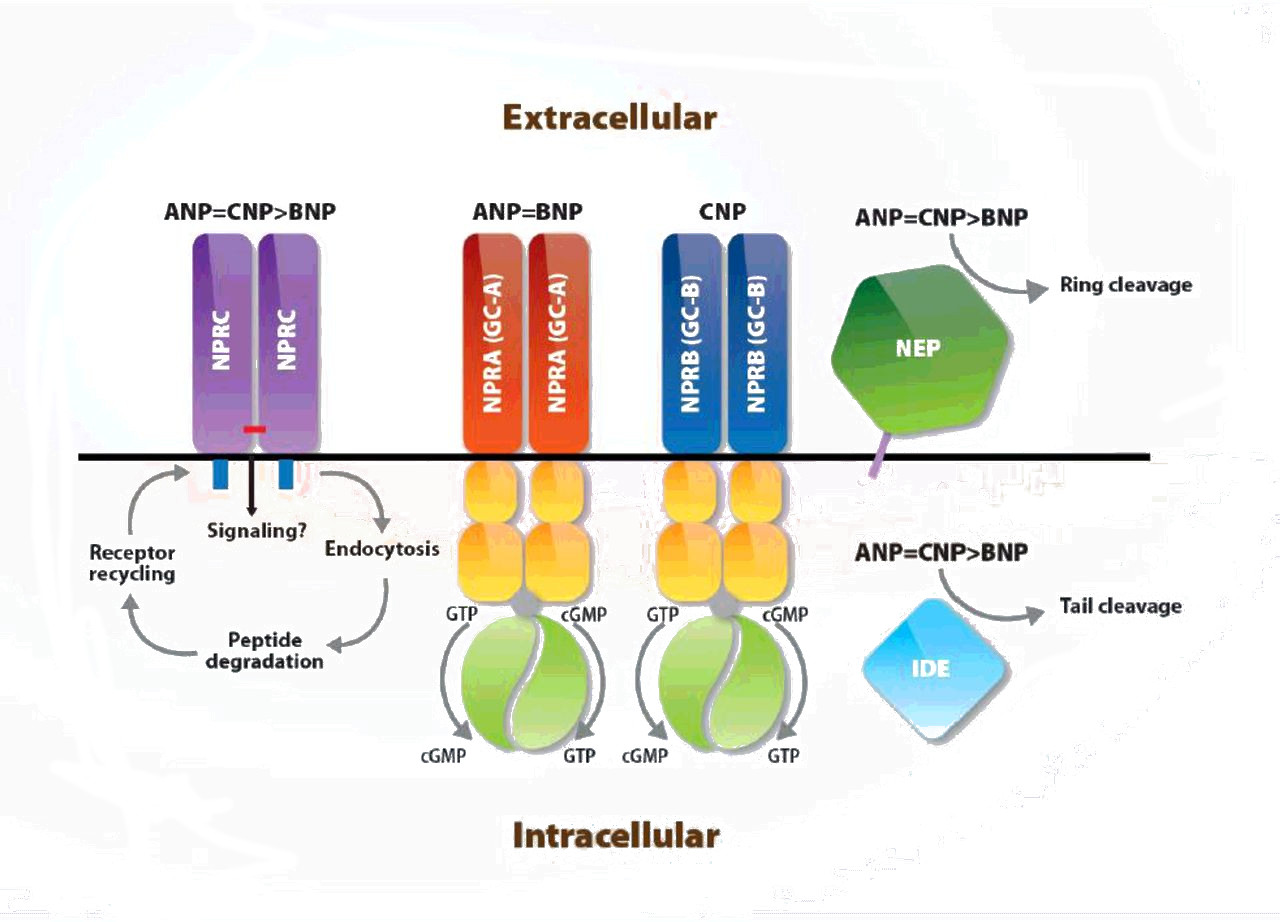
\includegraphics[scale=1]{../../images/NP_receptors.jpg}
    \small\caption{Schematic representation of natriuretic receptors}
    \label{NP_receptors}
\end{figure}


\subsubsection{Natriuretic Peptide Receptor-A}
Natriuretic peptide receptor-A (NPR-A) is the principal receptor of ANP and BNP.
%Its extracellular domain contains three intramolecular disulfide bonds and five N-linked glycosylation sites \citep{Miyagi2000a}.  NPR-A exists as a homodimer or homotetramer in its native state, and oligomerization is ligand-independent \citep{Chinkers1992} \citep{Iwata1991}, although ligand binding does bring the juxtamembrane regions of each monomer closer together \citep{Labrecque2001}.
NPR-A binds natriuretic peptides at a stoichiometry of 2:1 with a rank natriuretic peptide preference of: ANP $\ge$ BNP $>$ CNP \citep{Bennett1991} \citep{Koller1991} \citep{Suga1992a}.

Phosphorylation is essential for activation of NPR-A and dephosphorylation is a mechanism of desensitization in response to prolonged ANP exposure or protein kinase C activation \citep{Potter1992} \citep{Potter1994}. Although ATP increases ANP-dependent guanylyl cyclase activity, the mechanism for this effect is debatable \citep{Antos2005} \citep{Antos2007} \citep{Burczynska2007} \citep{Joubert2005}.  Data indicate that ATP reduces the Km for NPR-A \citep{Antos2007}.

NPR-A internalization and degradation is also controversial. One group consistently reports that the majority of internalized ANP-NPR-A complexes are degraded via a lysosomal pathway with a small portion returning intact to the plasma membrane \citep{Pandey2002}. Meanwhile, studies in primary kidney and Chinese Hamster ovary indicate that NPR-A is a membrane resident protein that does not undergo acute internalization and degradation \citep{Fan2005} \citep{Vieira2001}.

NPR-A and/or its mRNA is expressed in kidney, lung, adipose, adrenal, brain, heart, testis, and vascular smooth muscle tissue \citep{Goy2001}. NPR-A null mice exhibit chronic salt-resistant hypertension and cardiac hypertrophy and fibrosis \citep{Kuhn2002}.  A deletion in the human NPR-A gene was identified in nine Japanese individuals, of which eight had essential hypertension; the normotensive individual with the altered allele had left ventricular hypertrophy \citep{Nakayama2000}.  %To our knowledge, this study has not been repeated.

\subsubsection{Natriuretic Peptide Receptor-B}
Natriuretic peptide receptor-B (NPR-B) is the principal receptor of C-type natriuretic peptide (CNP) and exhibits similar topology, glycosylation, and intramolecular disulfide bonding patterns as NPR-A.\citep{Schulz1989}.
%The extracellular and intracellular regions of rat NPR-B are 43 and 78\% identical to rat NPR-A at the amino acid level, respectively

NPR-B binds natriuretic peptides with a selectivity preference of CNP $>$ ANP $\ge$ BNP \citep{Bennett1991} \citep{Koller1991} \citep{Suga1992a}.

NPR-B dephosphorylation has been shown to mediate desensitization in response to prolonged CNP exposure, protein kinase C activation, and intracellular calcium elevations \citep{Potter2000} \citep{Potthast2004}. ATP increases the guanylyl cyclase activity of NPR-B, by decreasing its Michaelis constant \citep{Antos2007}. NPR-B and/or its mRNA is expressed in bone, brain, fibroblasts, heart, kidney, liver, lung, uterine, and vascular smooth muscle tissue \citep{Bryan2006} \citep{Dickey2007}. Mice with a targeted disruption of the NPR-B gene, display dwarfism and  female sterility \citep{Tamura2004}.

NPR-B dominant negative mutant transgenic rats have also been generated. In addition to mild growth retardation of the long bones, the rats displayed progressive, blood pressure-independent cardiac hypertrophy and an elevated heart rate \citep{Langenickel2006}.

Consistent with a prominent role for CNP in the heart, NPR-B, not NPR-A, is the most active natriuretic peptide receptor in the failed heart \citep{Dickey2007}. Homologous loss-of-function mutations in human NPR-B result in a rare form of dwarfism called acromesomelic dysplasia, type Maroteaux (AMDM) \citep{Bartels2004}.

\subsubsection{Natriuretic Peptide Receptor-C}
Natriuretic peptide receptor-C (NPR-C) consists of a large extracellular ligand-binding domain that is approximately 30-35\% identical to NPR-A and NPR-B, a single membrane-spanning region, but only 37 intracellular amino acids \citep{Chang1989} \citep{Fuller1988} \citep{Porter1990}. It has no known enzymatic activity but has been  suggested to signal in a G protein-dependent manner \citep{Rose2008}.
It binds natriuretic peptides with a stoichiometry of two molecules of receptor to one molecule of ligand \citep{Ammarguellat2001}. Its ligand selectivity preference is: ANP $>$ CNP $\ge$ BNP \citep{Bennett1991} \citep{Suga1992a}.

The main function of NPR-C, also known as the clearance receptor, is to clear circulating natriuretic peptides through the process of receptor-mediated internalization and degradation \citep{Koh1992} \citep{Nussenzveig1990}. Internalization of NPR-C occurs in the absence of ligand; thus, this is a constitutive process \citep{Nussenzveig1990}. Osteocrin, an endogenous protein with limited homology to members of the natriuretic peptide family, binds NPR-C, but not NPR-A or NPR-B \citep{Moffatt2007}. Osteocrin is thought to compete with CNP for binding to NPR-C in bone, and therefore, increase local CNP levels during critical periods for bone development \citep{Moffatt2007}.

% NPR-C is the most widely and abundantly expressed natriuretic peptide receptor; for example, it constitutes \~94\% of the total ANP binding sites in endothelial cells \citep{Leitman1986}. NPR-C and/or its mRNA is expressed in adrenal, brain, heart, kidney, mesentery, and vascular smooth muscle tissue \citep{Nagase1997} \citep{Porter1990} \citep{Suga1992c} \citep{Wilcox1991}.
% NPR-C knockout mice exhibit increased ANP half-lives, long bone overgrowth, hypotension, mild diuresis, dilute urine, and blood volume depletion  \citep{Matsukawa1999}. Mouse strains containing chemically induced loss-of-function mutations in the extracellular domain of NPR-C display skeletal overgrowth from endochondral ossification defects as well \citep{Jaubert1999}.

\subsection{Physiologic Effects of Natriuretic Peptides}


\subsubsection{Natriuretic Peptide Effects on Blood Pressure}
ANP binding to NPR-A is a key-signaling pathway, which regulates normal homeostatic blood pressure. This is clearly demonstrated in mice lacking ANP or its receptor NPR-A, which have blood pressures that are elevated 20-40mmHg, compared to control mice \citep{John1995} \citep{John1996} \citep{Lopez1995} \citep{Oliver1997}.
The link between NPR-A and blood pressure in mice is particularly strong because Smithies and colleagues demonstrated that NPR-A copy number is inversely related to blood pressure in a  remarkably linear manner \citep{Oliver1998}.
Conversely, blood pressures in transgenic mice overexpressing ANP or BNP are substantially decreased \citep{Ogawa1994a} \citep{Steinhelper1990}. Although infusion of supraphysiological levels of CNP into animals acutely decreases blood pressure \citep{Clavell1993} \citep{Sudoh1990}, mice lacking functional CNP or NPR-B are normotensive \citep{Chusho2001} \citep{Tamura2004}, suggesting that the CNP/NPR-B pathway is not a fundamental regulator of basal blood pressure in mice.

NPR-A dependent decreases in blood pressure are achieved through natriuresis and diuresis, vasorelaxation, increased endothelium permeability, and antagonism of the renin-angiotensin system. Classic experiments showed that atrial extract infusions resulted in rapid renal excretion of water and sodium \citep{deBold1981}. Studies by Garbers and colleagues indicated that the renal response requires NPR-A because mice lacking this receptor do not respond to ANP, BNP, or to acute volume expansion \citep{Kishimoto1996}. Similar studies found that NPR-A was also required for ANP- or BNP-dependent vasorelaxation in mice \citep{Lopez1997}. Physiological experiments involving mice with severe reductions of NPR-A in vascular smooth muscle cells demonstrated that while smooth muscle NPR-A is required for acute ANP- or BNP-dependent vasorelaxation, this response does not play a significant role in controlling chronic blood pressure \citep{Holtwick2002}.

The ability of the ANP/NPR-A pathway to increase  endothelial permeability is supported by the observation that hematocrit levels are elevated prior to urination and are preserved in nephrectomized animals \citep{Almeida1986} \citep{Fluckiger1986} \citep{Richards1988}.
 Furthermore, mice with genetically engineered reductions of NPR-A in vascular endothelium exhibit volume expansion, hypertension, and reduced albumin clearance from the vascular system \citep{Sabrane2005}.

\subsubsection{Effects of Natriuretic Peptides on Cardiac Hypertrophy and Fibrosis}

Although prolonged hypertension can cause hypertrophy, the level of hypertrophy in NPR-A deficient mice is significantly greater than that observed in other genetic models that cause similar levels of hypertension, suggesting that NPR-A elicits a local growth inhibitory signal in the heart. Data for this idea was initially shown in NPR-A knockout mice, which have enlarged hearts even when effectively treated with antihypertensive drugs from birth \citep{Knowles2001}. Additional studies determined that transgenic re-expression of NPR-A in the hearts of NPR-A -/- mice reduced cardiomyocyte size without affecting heart rate or blood pressure \citep{Kishimoto2001}.
Finally, mice with reduced cardiomyocyte expression of NPR-A exhibited moderate hypertrophy even though they were slightly hypotensive \citep{Holtwick2003} \citep{Patel2005}. %In terms of natriuretic peptides, mice lacking ANP have larger hearts, whereas mice transgenically overexpressing ANP have smaller hearts \citep{Barbee1994} \citep{Steinhelper1990}.
In contrast, targeted deletion of BNP resulted in normotensive mice with normal heart size but with increased ventricular fibrosis - especially when subjected to pressure overload \citep{Tamura2000}. Thus, genetic studies in mice strongly support a role for ANP activation of NPR-A in the local inhibition of cardiac hypertrophy and BNP activation of NPR-A in the inhibition of cardiac fibrosis.

Data supporting a role for the CNP/NPR-B pathway in cardiac remodeling has been reported. Although NPR-B inactivation mutations in mice have not been shown to cause hypertrophy \citep{Tamura2004} \citep{Tsuji2005}, transgenic rats expressing a dominant negative form of NPR-B exhibit mild blood pressure-independent cardiac hypertrophy and increased heart rate \citep{Langenickel2006}.
In addition, CNP infusion was shown to reduce cardiac remodeling in response to experimentally induced myocardial infarction in rats, and transgenic expression of CNP improved outcomes in mice subjected to ischemia/reperfusion injury or myocardial infarction \citep{Wang2007}.

\subsubsection{Effects of CNP and NPR-B on Bone Growth}
The most obvious function of the CNP/NPR-B pathway is to stimulate long bone growth. Though undetectable at birth, mice lacking functional CNP or NPR-B develop dwarfism due to impaired endochondrial ossification \citep{Chusho2001} \citep{Tamura2001} \citep{Tsuji2005}.
Conversely, transgenic CNP overexpression or reduced degradation of CNP due to loss-of-function mutations in NPR-C result in skeletal overgrowth \citep{Yasoda2004}. Growth plate histology reveals that the endochondral proliferative and hypertrophic zones are reduced in mice with impaired CNP or NPR-B signaling, whereas overexpressing mice have enlarged growth plates \citep{Chusho2001} \citep{Tamura2004} \citep{Yasoda2004}.

One cGMP effector involved in the long bone growth pathway is cGMP-dependent protein kinase II, also known as PKGII or cGKII. Loss-of-function mutations in the mouse or rat gene that encodes this kinase also cause dwarfism \citep{Chikuda2004} \citep{Pfeifer1996}. Interestingly, the growth plates of rodents with defective cGKII are enlarged, which differs from the diminished growth plates seen in the CNP or NPR-B deleted mice, suggesting that a cGKII-independent pathway is also involved in CNP-dependent long bone growth.

Humans with two loss-of-function alleles for NPR-B suffer from a rare type of autosomal recessive dwarfism, called acromesomelic dysplasia, type Maroteaux \citep{Bartels2004}. These individuals are characterized by disproportionate limb to torso ratios that are only obvious a year or more after birth. Interestingly, although single copy carriers of a nonfunctional NPR-B allele do not suffer from disease, they are statistically shorter than comparable individuals with two wild type NPR-B alleles \citep{Olney2006}. %Thus, it is possible that NPR-B mutations could have a significant effect on the stature of the general population.

\subsection{Biological Action of CNH }

Cardiac natriuretic hormones have powerful physiological effects on the cardiovascular system, body fluid, and electrolyte homeostasis \citep{13} \citep{28} \citep{30} \citep{77} \citep{78}. CNH share a direct diuretic, natriuretic and vasodilator effect and an inhibitory action on ventricular myocyte contraction \citep{79} as well as remodeling and inflammatory processes of myocardium and smooth muscle cells \citep{80} \citep{81} \citep{82} \citep{83} (Fig. 3.14). Thus, CNH exert a protective effect on endothelial function by decreasing shear stress, modulating coagulation and fibrinolysis pathways, and inhibiting platelet activation (Fig. 3.15). They can also inhibit vascular remodeling process as well as coronary restenosis post-angioplasty \citep{56} \citep{84} \citep{85} \citep{86} \citep{87} \citep{88} \citep{89}.

% CNH share an inhibitory action on neuro-hormonal and immunological systems, and on some growth factors. In particular, the pivotal role of CNH (especially ANP) in modulating the immune response has been reviewed \citep{98}.
The first evidence for a role of CNH in the immune system was given by the fact that peptide hormones and their receptors are expressed in various immune organs. Furthermore, several studies indicated that the CNH system in immune cells underlies specific regulatory mechanisms by affecting the innate as well as the adaptive immune response. In particular, ANP increases phagocytotic activity and production of reactive oxygen species of phagocytes. ANP affects the induced innate immune response by regulating the activation of macrophages at various stages. It also reduces production of pro-inflammatory medi ators by inhibition of iNOS and COX-2 as well as TNF-\alpha synthesis. ANP also affects TNF-\alpha action, i.e. it interferes with the inflammatory effects of TNF-\alpha on the endothe lium. The peptide hormone counteracts TNF-\alpha-induced endothelial permeability and adhesion and attraction of inflammatory cells. Finally, it affects thymopoesis and T cell maturation by acting on dendritic cells and regulates the balance between TH1 and TH2 responses \citep{99}.

The cited effects on the cardiovascular system and body fluid and electrolyte homeostasis can be explained at least in part by the inhibition of control systems, including the sym pathetic nervous system, the renin-angiotensin-aldosterone system (RAAS), the vaso pressin/antidiuretic hormone system, the endothelin system, cytokines and growth factors \citep{90} \citep{91} \citep{92} \citep{93} \citep{94} \citep{95} \citep{96} \citep{97} \citep{98} \citep{99}.The endocrine action,shared by plasma ANP and BNP,can be enhanced by natriuretic peptides produced locally in target tissues (paracrine action). Indeed, endothelial cells syn thesize CNP, which in turn exerts a paracrine action on vessels \citep{57} \citep{84} \citep{85} \citep{86} \citep{87} \citep{88}. Moreover, renal tubular cells produce urodilatin, another member of the peptide natriuretic family, which has powerful diuretic and natriuretic properties \citep{100}.Genes for natriuretic peptides (includ ing ANP, BNP and CNP) are also expressed in the central nervous system, where they likely act as neurotransmitters and/or neuromodulators \citep{91} \citep{92} \citep{93} \citep{100} \citep{101} \citep{102}. In particular, it was demonstrated that intranasal ANP acts as central nervous inhibitor of the hypothalamus pituitary-adrenal stress system in humans \citep{103}. Finally, co-expression of CNH and of their receptors was observed in rat thymus cells and macrophages \citep{104} \citep{105},suggesting that CNH may have immunomodulatory and anti-inflammatory functions in mammals \citep{106}.

A  detailed review \citep{107} has highlighted a possible major role for CNH in the development of certain systems, in particular skeleton, brain, and vessels. This review cites  studies showing severe skeletal defects and impaired recovery after vascu lar and renal injury in CNH transgenic and knockout (KO) mice \citep{108}. In addition, CNH may have a role in the regulation of proliferation, survival, and neurite outgrowth of cultured neuronal and/or glial cells \citep{108}.

Changes in plasma ANP are also correlated with alcohol-associated psychological vari ables \citep{108}. Acute administration of alcohol stimulates the release of ANP independent ly of volume-loading effects. Patients whose ANP levels fell markedly during abstinence also reported more intense and frequent craving as well as more anxiety \citep{108}.  Several reports have shown that CNH stimulate the synthesis and release of testos terone in a dose-dependent manner in isolated and purified normal Leydig cells \citep{109} \citep{112}. It has been suggested that this effect on normal Leydig cell steroidogenesis does not involve classical mechanisms of cAMP-mediated regulation of steroidogenic activ ity by gonadotropins \citep{112}. The stimulated levels of testosterone production by ANP, BNP, and gonadotropins were comparable, whereas CNP has been found to be a weak stim ulator of testosterone production in Leydig cells \citep{112}. Moreover, testicular cells contain immunoreactive ANP-like materials and a high density of natriuretic peptide recep tor-A (NRP-A) \citep{112}. These findings suggest that CNH play paracrine and/or autocrine roles in testis and testicular cells. Furthermore, the presence of ANP and its receptors has been reported in ovarian cells, too. Increasing evidence strongly support that CNH are present and probably locally synthesized in ovarian cells of different mammalian species and also play an important physiological role in stimulating estradiol synthe sis and secretion in the female gonad \citep{112} \citep{113} \citep{114} \citep{115}. However, further studies are necessary in order to clarify completely the role played by CNH in the regulation of gonadal func tion and also to assess the inter-relationship between heart endocrine function and gonadal function in humans.

The huge amount of data reported above strongly supports the hypothesis that CNH are active components of the body integrative network that includes nervous, endocrine and immune systems. According to this hypothesis, the heart can no longer be seen as a passive automaton driven by nervous, endocrine or hemodynamic inputs, but as a leading actor on the stage. Thus, CNH, together with other neuro-hormonal factors, regulate cardiovascular hemodynamics and body fluid and electrolyte homeostasis, and probably modulate inflammatory response in some districts, including the car diovascular one. This hypothesis implies that there are two counteracting systems in the body: one has sodium-retaining, vasoconstrictive, thrombophylic, pro-inflamma tory and hypertrophic actions, while the second one promotes natriuresis and vasodi latation, and inhibits thrombosis, inflammation and hypertrophy. CNH are the main effectors of the latter system, and work in concert with NO, some prostaglandins, and other vasodilator peptides (such as bradykinin) \citep{116} \citep{117} \citep{118} \citep{119} \citep{120}. Under physiological condi tions, the effects of these two systems are well balanced via feedback mechanisms, and result in a beat-to-beat regulation of cardiac output and blood pressure in response to endogenous and exogenous stimuli. In patients with HF, the action of the first system is predominant, as a compensatory mechanism, initially, that progressively leads to detrimental effects.

The knowledge so far accumulated regarding CNH suggests that a continuous and intense information exchange flows from the endocrine heart system to nervous and immunological systems and to other organs (including kidney, endocrine glands, liver, adipose tissue, immuno-competent cells) and vice versa (Fig. 3.16). From a pathophys iological point of view, the close link between the CNH system and counter-regulatory systems could explain the increase in circulating levels of CNH in some non-cardiac-relat ed clinical conditions. Increased or decreased BNP levels were frequently reported in acute and chronic respiratory diseases \citep{121} \citep{122} \citep{123} \citep{124} \citep{125} \citep{126} \citep{127} \citep{128} \citep{129}, some endocrine and metabolic diseases \citep{130} \citep{131} \citep{132} \citep{133} \citep{134} \citep{135} \citep{136} \citep{137} \citep{138} \citep{139} \citep{140} \citep{141}, liver cirrhosis \citep{142} \citep{143} \citep{144}, renal failure \citep{100} \citep{144}, septic shock, chronic inflam matory diseases \citep{145} \citep{146} \citep{61} \citep{148} \citep{149}, subarachnoid hemorrhage \citep{150} \citep{153} \citep{152}, and some paraneo plastic syndromes \citep{154} \citep{155} \citep{156}. In addition, any myocardial damage leading to the release of sarcoplasma constituents (including CNH) in extracellular fluid, for instance that due to cardiotoxic agents \citep{157} \citep{158} \citep{159} \citep{160} \citep{161}, cardiac trauma or ischemic necrosis \citep{162} \citep{163}, also causes an increase in plasma concentration of CNH.

Furthermore, the inter-relationships between the CNH system and pro-inflammatory cytokines suggest that cardiac hormones play an important role in mechanisms respon sible for cardiac and vascular adaptation, maladaptation and remodeling in response to various physiological and pathological stimuli \citep{32} \citep{35} \citep{62} \citep{162}.  Elevated BNP levels in extra-cardiac diseases reveal an endocrine heart response to a “cardiovascular stress” (Fig. 3.17). Indeed,  studies reported that plasma BNP concentration is an independent risk factor for mortality (cardiac and/or total) in pul monary embolism \citep{121} \citep{123} \citep{124} and hypertension \citep{127}, renal failure \citep{28} \citep{100} \citep{144}, sep tic shock \citep{145}, amyloidosis \citep{149}, and diabetes mellitus \citep{141} (see Chapter 6 for more details). According to this hypothesis, a BNP assay should be considered as a marker of cardiac stress (Fig. 3.17).

In conclusion, CNH share a powerful action on the cardiovascular system, including diuretic, natriuretic and vasodilator effects and an inhibitory action on ventricular myocyte contraction, as well as on remodeling and inflammatory processes of myocardi um and smooth muscle cells. Furthermore, CNH exert a protective effect on endothelial function by decreasing shear stress, modulating coagulation and fibrinolysis pathways, and inhibiting platelet activation. They can also inhibit the vascular remodeling process as well as coronary restenosis post-angioplasty. These effects can be explained, at least in part, by the inhibition of control systems, including the sympathetic nervous system, the RAAS, the vasopressin/antidiuretic hormone system, the endothelin system, cytokines and growth factors. Finally, the endocrine action of ANP and BNP is potentiated at the periphery (target tissues) by the paracrine action of other members of the peptide natri uretic family, such as CNP (in the vascular tissue) and urodilatin (in renal tissue).  Finally, some experimental studies performed in KO mice suggest a distinct patho physiological role for BNP in respect to ANP \citep{18}. While BNP KO mice are no different from control mice with regard to blood pressure, urine volume, and urinary electrolyte excretion, they have more extensive ventricular fibrosis, accompanied by increased transforming growth factor-b3 (TGF-b3) and collagen mRNA \citep{18}. These data suggest that BNP may function more as an autocrine/paracrine inhibitor of cell growth in the heart; while ANP may be considered as a traditional circulating hormone with pro nounced diuretic, natriuretic, and antihypertensive effects.

\subsection{Natriuretic Peptide Receptors and Intracellular Second Messenger Signaling}
Cardiac natriuretic hormones share their biological action by means of specific recep tors (NPR), which are present within the cell membranes of target tissues. Three different subtypes of NPRs have so far been identified in mammalian tissues \citep{112} \citep{164} \citep{165}.

\subsubsection{Genes Encoding for NPRs}
NPR1 is the gene coding the NPR-A receptor (natriuretic peptide receptor A/guany late cyclase A) and it is located on 1q21-q22 spanning 15,534 bp with 22 exons. The rel ative mRNA of 3,805 bp leads to a protein of 1,061 amino acids.  The NPR-B receptor (natriuretic peptide receptor B/guanylate cyclase B) is codified by the gene NPR2. This gene of 17,303 bp is on chromosome 9 (9p21-p12) and it is organized in 22 exons, which can give two types of mRNA. NPR2 Ia is an mRNA of 3,482 bp that has a 71 nucleotide insertion relative to isoform b, which results in a dif ferent, and shorter (995 aa), carboxy-terminus that may disrupt the guanylyl cyclase activity. NPR2 Ib (3,411 bp, 1,047 aa) does not include the alternate exon found in iso form a, and thus isoform b contains a longer carboxy-terminus. The natriuretic peptide receptor C gene, also named NPR3, is on 5p14-p13 and spans 74,698 bp (8 exons), giv ing an mRNA of 1,753 bp that is translated into a protein of 540 amino acids.

\subsubsection{Biological Function of NPRs}
NPR-A and NPR-B are generally considered to mediate all known biological actions throughout the guanylate cyclase (GC) intracellular domain, while the third member of the natriuretic peptide receptor family, the NPR-C receptor, does not have a GC domain (Figs. 3.18, 3.19 and 3.20).  The GC receptors for ANP/BNP (NPR-GC-A) and CNP (NPR-GC-B) belong to a fam ily of seven isoforms of transmembrane enzymes (from GC-A to GC-G), which all con vert guanosine triphosphate into the second messenger cyclic 3’,5’-guanosine monophos phate (cGMP) \citep{164}.

Although partly homologous to soluble GC, the receptor for NO, the membrane GCs share a different and unique topology. The single transmembrane span domain divides the protein structure into an extracellular ligand binding domain and an intracellular region consisting of a protein kinase-homology domain, an amphipathic helical or hing region, and a cyclase-homology domain \citep{165} (Figs. 3.18, 3.19 and 3.20). The cyclase homology domain represents the catalytic cGMP synthesizing domain. The function of the intracellular region consisting of a protein kinase-homology domain is incom pletely understood. Although it probably binds ATP and contains many residues con served in the catalytic domain of protein kinases, kinase activity has not been detect ed \citep{165}. It represses the enzyme activity of the catalytic cGMP-synthesizing domain and at the same time is necessary for its ligand-dependent activation \citep{154}. The coiled-coil hing region is involved in receptor dimerization, which is also essential for the activa tion of the catalytic domain \citep{165}.

The cGMP produced modulates the activity of specific downstream regulatory pro teins, such as cGMP-regulated phosphodiesterases, ion channels and cGMP-dependent protein kinases type I (PKG I) and type II (PKG II) (Fig. 3.20). These proteins should be considered to be third messengers, which are differentially expressed in different cell types, ultimately modifying cellular functions \citep{166} \citep{167}. This specific action of CNH on target tissues depends essentially on two different mechanisms.

The physiological expression of NPR-A and NPR-B differs quite significantly in human tissues (Fig. 3.21). NPR-A is found in abundance in larger, conduit blood vessels, whereas the NPR-B is found predominantly in the central nervous system \citep{168}. Both receptors have been localized in adrenal glands and kidney \citep{168}. On the other hand, several studies indicate that phosphorylation of the kinase homology domain is a crit ical event in the regulation of NPRs \citep{169} \citep{170} \citep{171}.

The affinity for ANP, BNP and CNP also varies greatly among the different NPRs.  ANP shows a greater affinity for NPR-A and NPR-C, and CNP for NPR-B, while BNP shows a lower affinity for all NPRs compared to the other two peptides (Fig. 3.21).  Activation of the GC-linked NPRs is incompletely understood \citep{172}. NPR-A and NPR B are homo-oligomers in the absence and presence of their respective ligands, indicat ing that receptor activation does not simply result from ligand-dependent dimerization \citep{173}. However, ANP binding does cause a conformational change of each monomer closer together \citep{172} \citep{173} \citep{174} \citep{175} \citep{176}. The stoichiometry of the ligand-receptor complex is 1:2 \citep{177}.  Initial in vitro data suggested that direct phosphorylation of NPR-A by protein kinase C mediated its “desensitization” (i.e., the process by which an activated receptor is turned off) \citep{178}. However, subsequent studies conducted in live cells indicated that desensiti zation in response to prolonged natriuretic peptide exposure or activators of protein kinase C results in a net loss of phosphate from NPR-A and NPR-B \citep{171} \citep{179} \citep{180} \citep{181} \citep{182}.

Although ligand-dependent internalization and degradation of NPR-A has been intense ly studied by several groups for many years, a consensus understanding of the importance of this process in the regulation of NPRs has not emerged \citep{182}. Early studies conducted on PC-12 pheochromocytoma cells suggested that both NPR-A and NPR-C internalize ANP and that both receptors are recycled back to the cell surface \citep{184}. Other studies, using Leydig, Cos, and 293 cell lines, have reported that ANP binding to NPR-A stimulates its internalization, which results in the majority of the receptors being degraded with a smaller portion being recycled to the plasma membrane \citep{184} \citep{185} \citep{186} \citep{187}. In contrast, other stud ies performed in cultured glomerular mesangial and renomedullary interstitial cells from the rat or Chinese hamster ovary cells reported that NPR-A is a constitutively membrane resident protein that neither undergoes endocytosis nor mediates lysosomal hydrolysis of ANP \citep{188} \citep{189}. A more  study using 293T cells suggested that NPR-A and NPR B are neither internalized nor degraded in response to receptor occupation \citep{173}. Fur thermore, this study did not support the hypothesis that down-regulation is responsible for NPR desensitization observed in response to various physiological or pathological stim uli \citep{182}.Further studies are necessary to clarify whether or not ANP binding to NPR-A stim ulates its internalization, and whether this process is tissue- and/or species-specific.

It is generally thought that the NPR-C is not linked to GC and so serves as a clearance receptor \citep{28} \citep{77} \citep{78}.NPR-C is present in higher concentration than NPR-A or NPR-B in sev eral tissues (especially vascular tissue),and it is known constitutively to internalize CNH \citep{172} (Fig.3.22).However, studies have found that CNH interact with NPR-C to suppress the cAMP concentration by inhibition of adenylyl cyclase \citep{190} \citep{191}. Specific binding to NPR-C increases inositol triphosphate and diacylglycerol concentrations by activating phospholi pase C activity or inhibits DNA synthesis stimulated by endothelin, platelet-derived growth factor and phorbol ester by inhibiting MAPK activity,as  reviewed \citep{190}.The NPR-C mediated inhibition of adenylyl cyclase is mediated through Gi (inhibitory guanine nucleotide regulatory) proteins.According to this hypothesis,NPR-C,which is present in large amounts, especially on the endothelial cell wall,may mediate some paracrine effects of CNP on vascu lar tissue \citep{168} \citep{190}.However,further studies are necessary to elucidate the possible role of NPR C receptors as modulators of CNH action and/or degradation in peripheral tissues.

\subsection{Metabolic Pathways and Circulating Levels of CNH}
Atrial natriuretic peptide and BNP are secreted directly from the heart. In the circula tion, CNHs are metabolized via two principal mechanisms: degradation by a membrane-bound endopeptidase (NEP 24.11) and receptor-mediated cellular uptake via NPR-C \citep{14} (Fig. 3.22). Some biological characteristics of ANP, BNP and CNP (as well as of their precursors) are summarized in Table 3.3.

\subsubsection{ANP Metabolism}
Atrial natriuretic peptides are a family of peptides derived from a common precursor, called preproANP, which in humans contains 151 amino acids and has a signal peptide sequence at its amino-terminal end (Fig. 3.11). The pro-hormone is stored in secretion granules of cardiomyocytes as a 126-amino-acid peptide, proANP 1-126 , which is pro duced by cleavage of the signal peptide. When appropriate signals for hormone release are given, proANP 1-126 is further split by some proteases (especially the serine protease corin) \citep{192} into N-terminal fragment NT-proANP and the COOH-terminal peptide ANP, which is generally considered to be the biologically active hormone, because it contains the cysteine ring (Figs. 3.1 and 3.11).

Studies from the group of Vesely et al. suggested that the NT-proANP can be metab olized in vivo in three peptide hormones with blood pressure-lowering, natriuretic, diuretic and/or kaliuretic properties \citep{100}. These peptide hormones, numbered by their amino acid sequences, beginning at the N-terminal end of the proANP pro-hormone, include: 1) the peptide proANP 1-30 , also called long-acting natriuretic peptide (LANP); 2) the peptide proANP 31-67 with vessel dilator properties; 3) the peptide proANP 79-98 with kaliuretic properties \citep{98}. However, these three peptides do not bind to the same NPRs of CNHs, because they do not have the cysteine ring. Further studies are neces sary to confirm and elucidate the biological action of these putative peptide hormones, as well as their in vivo metabolism.

There is some evidence that ANP is secreted according to a pulsatile pattern in humans \citep{193} \citep{194} \citep{195} \citep{196} \citep{197}. Upon secretion, ANP is rapidly distributed and degraded (the metabolic clearance rate of ANP is on average about 2,000 ml/min in healthy subjects) with a plasma half-life of about 4-6 minutes in healthy adult subjects. In humans, about 50\% of the ANP secreted into the right atrium is extracted by the peripheral tissues during the first pass throughout the body \citep{198} \citep{199} \citep{200} \citep{201}. Furthermore, circulating ANP represents only a small fraction of the total body pool (no more than 1/15) in normal subjects and plasma ANP concentration shows rapid and wide fluctuations in healthy subjects, even at rest in the recumbent position \citep{198} \citep{199} \citep{200} \citep{201}. The turnover data suggest that circulating levels of ANP may not represent a close estimate of their disposal, and therefore of the activity of the CNH system, as implicitly accepted in physiological or clinical studies in which only the plasma concentration of the hormone is measured, without an estima tion of turnover rate. However, it was demonstrated that ANP clearance mechanisms are constant in the presence of rapid and large changes in endogenous ANP plasma levels induced by atrial and/or ventricular pacing, thus indicating that, at least for studies lasting only a few hours, changes in ANP circulating levels may provide a reliable esti mate of production rate variations \citep{201}.

\subsubsection{BNP Metabolism}
The biological action, metabolic pathways, and turnover parameters of BNP are not as well known as those of ANP \citep{14}. However, it is commonly believed that the BNP turnover is less rapid than that of ANP with a plasma half-life of about 13-20 min utes; indeed, circulating levels of BNP are more stable than those of ANP in adult healthy subjects (Fig. 3.23). Bentzen et al. \citep{197} analyzed the secretion pattern of ANP and BNP in 12 patients with chronic HF and in 12 healthy adult subjects. ANP and BNP in plasma were determined by radioimmunoassay (RIA) at 2 min intervals during a 2-h period and were subsequently analyzed for pulsatile behavior using the method of Fourier transformation. All patients and healthy subjects had significant rhythmic oscillations in plasma ANP levels, and 11 patients with HF and 10 healthy subjects had significant rhythmic oscillations in plasma BNP levels \citep{197}. The ampli tude of the main frequency was considerably higher in patients than in healthy sub jects, but the main frequency did not differ significantly between patients and healthy subjects for either ANP or BNP. Patients with HF demonstrated pulsatile secretion of ANP and BNP with a much higher absolute amplitude, but with the same main fre quency as healthy subjects \citep{197}. Finally, rhythmic oscillations in plasma ANP lev els of healthy subjects showed significantly higher mean amplitude, but not fre quency, than those of BNP \citep{197}.

A very small amount of immunoreactive BNP has been found in urine \citep{202} \citep{203}, but the precise mechanism of renal excretion has not yet been fully clarified. In contrast to BNP, the biologically active peptide, other proBNP-derived inactive fragments also cir culate in plasma. These fragments are commonly referred to as “N-terminal proBNP” (NT-proBNP), but the molecular heterogeneity also includes the intact precursor, par ticularly in patients with HF \citep{14} \citep{204}. Cardiac secretion of proBNP and its N-termi nal fragments has been demonstrated by blood sampling from the coronary sinus \citep{205}.  Some data suggest that the major part of proBNP produced in myocardiocytes is appar ently processed prior to release \citep{14}; however, intact proBNP peptide was also found in plasma of patients with HF as well as healthy adult subjects \citep{14} \citep{205} \citep{206}.

A  study, employing a new method for the total and equimolar assay of all proB NP-related peptides (i.e., intact proBNP precursor plus NT-proBNP concentrations), found comparable peripheral concentrations of BNP (measured by immunoradiomet ric assay) and proBNP-related peptides in patients with HF \citep{206}. Moreover, the BNP concentration (median 125 pmol/l) was higher than that of total proBNP (103 pmol/l) in the coronary sinus, suggesting that the cardiac secretion of these two peptides could be different \citep{206}.Alternatively, this finding could also reflect some difference in peripheral elimination of peptides because total proBNP concentration is significantly higher in the pulmonary artery than the aortic root in patients with right ventricular failure \citep{207}.

While NEP enzymes are mainly involved in natriuretic peptide inactivation in vivo, the degradation of BNP seen in vitro is most likely due to other enzymes, such as peptyl arginine aldehyde proteases, kallikrein, and serine proteases \citep{15}. However, the role of these enzymes in the degradation of BNP in vivo is unclear.

A  study reported that both the BNP and total proBNP concentrations were increased more than 2-fold in the coronary sinus compared to the inferior caval vein (BNP-32: median 125 pmol/l, range 21-993 vs median 52 pmol/l, range 7-705; proBNP: median 103 pmol/l, range 16-691 vs 47 pmol/l, 8-500) \citep{206}. These findings are in accordance with previous studies suggesting that the cardiac gradient for BNP secre tion (as estimated by the difference between BNP concentration in coronary sinus and inferior caval vein) ranges from 1.6-fold to 2.9-fold \citep{204} \citep{208} \citep{209} \citep{210}. Taking these studies as a whole, ANP and BNP share a similar peripheral extraction value (of about 30-50\%). Further studies are necessary to elucidate the metabolism of BNP and in particular the predominant form of the circulating BNP-related peptides.

\subsection{CNH Genes and Cardiovascular Diseases}
Since CNH have a potent diuretic antihypertensive action, and the impaired action of the peptides may cause hypertension, their genes may be candidates for cardiovascu lar disease, especially arterial hypertension. Furthermore, transgenic animals (espe cially mice), overexpressing CNH or knockout for ANP/BNP genes or their specific receptors, have been used to evaluate the pathophysiological role of the CNH system in cardiovascular diseases \citep{251}.

In transgenic mice with overexpression of ANP and BNP in liver, plasma ANP and BNP levels are from 10- to 100-fold higher than in control mice, with a blood pressure of 20-25 mmHg lower. These mice also have lighter hearts, but with the same cardiac out put and rate, than controls \citep{251} \citep{253} \citep{254} \citep{255}. The BNP-overexpressing mice show the same hemodynamic changes; on the other hand, ANP KO mice develop NaCl-sensitive hyper tension \citep{251}. Transgenic mice overexpressing the NPRA gene have also been created; these animals have a lower blood pressure than wild-type mice \citep{251}. The correspon ding KO mice show an increase in blood pressure compared with controls (on average 10 mmHg in heterozygous and 30 mmHg in homozygous animals), which is not affect ed by NaCl intake \citep{254} \citep{255}. These data suggest a different pathophysiological mech anism for hypertension between KO mice for the ANP gene and its specific receptor; this difference does not yet have an explanation \citep{251}. NPRC heterozygous KO mice do not show blood pressure variation, whereas homozygous mice show on average a decrease in blood pressure of about 8 mmHg \citep{251}.

The function of natriuretic peptides was also studied after induction of myocardial infarction in KO mice lacking the natriuretic peptide receptor guanylyl cyclase-A, the receptor for ANP and BNP \citep{89}. KO and wild-type mice were subjected to left coronary artery ligation and then followed-up for 4 weeks. KO mice showed significantly higher mortality because of a higher incidence of acute HF, which was associated with dimin ished water and sodium excretion and with higher cardiac levels of mRNAs encoding ANP, BNP, TGF-b1, and type I collagen. By 4 weeks after infarction, left ventricular remodeling, including myocardial hypertrophy and fibrosis, and impairment of left ventricular systolic function were significantly more severe in KO than wild-type mice \citep{89}. These data confirm that the CNH system has powerful anti-remodeling properties on ventricular cardiomyocytes.

In  years, molecular genetic techniques have been introduced in etiological stud ies of polygenetic diseases, in linkage studies, in sib-pair linkage studies of various candi date genes, and in related studies \citep{251} \citep{252}. The association between some abnormalities in genes, coding for the CNH and their receptors, and some cardiovascular (in particular hypertension) and metabolic (such as diabetes mellitus) diseases has been tested in a large number of clinical studies (see also Chapter 6 for more details). To date, the results obtained are conflicting and seem to depend strictly on the ethnic population of the study.  The restriction fragment length polymorphism for the enzyme HpaII, located in intron 2 of NPPA (polymorphism also called Sma I), was reported to be more common in hypertensive African-Americans than in normotensive black controls \citep{257}; these data were then confirmed in two \citep{258} \citep{259}, but not a third \citep{260}, Caucasian popula tions. Furthermore, another study found that the HpaII polymorphism was not asso ciated with hypertension in the Chinese population of Hong Kong \citep{261}.

Regarding other NPPA polymorphisms, Japanese studies reported that both G1837A and T2238C polymorphisms are associated with essential hypertension \citep{262}, while only a marginally significant association was found with an ANP polymorphism locat ed in the 5’-untranslated region (C664G) \citep{263}.

Several allelic variants have also been described for genes coding for CNH recep tors (see the  revew by Nakayama \citep{251} for a more detailed discussion of this topic). The clearance receptor for natriuretic peptides (NPR-C) is highly expressed in adipose tissue, and its bi-allelic (A/C) polymorphism was detected at position -55 in the conserved promoter element named P1. This variant of the NPR-C P1 promoter is associated with lower ANP levels and higher systolic blood pressure and mean blood pres sure in obese hypertensives: the C(-55) variant, in the presence of increased adiposity, might reduce plasma ANP through increased NPR-C-mediated ANP clearance, con tributing to higher blood pressure \citep{264}.

In the Japanese population an insertion/deletion (GCTGAGCC) polymorphism has been identified in the 5’-flanking region of the NPRA gene that is associated with essen tial hypertension and left ventricular hypertrophy \citep{265}. Another insertion/deletion polymorphism is on the 3’-untranslated region of the NPRA gene, on exon 22, and it seems to be associated with familial hypertension \citep{266}. However, these data should be confirmed in larger studies, including other ethnic populations.

3.9 An Integrated Neuro-Hormonal System Regulates Vascular Function

Endothelial cells release an array of vasoactive mediators that alter the tone and growth of the underlying smooth muscle and regulate the reactivity of circulating white blood cells, erythrocytes and platelets. These endogenous factors are usually called endothe lium-derived vasorelaxant mediators \citep{267}. Moreover, it appears that alterations in the capacity of the endothelium to release some mediators in response to pathophysiolog ical stimuli (the so-called endothelium dysfunction) are a major precipitating factor in many cardiovascular diseases. Perhaps the most important of these paracrine medi ators are prostacyclin (PGI 2 ) and nitric oxide (NO). More , a third endotheli um-derived vasorelaxant mediator has been described \citep{267}. This is termed endothe lium-derived hyperpolarizing factor (EDHF) because it elicits a characteristic smooth muscle hyperpolarization and relaxation. Much attention has focused on identifying EDHF(s), with diverse candidates, including cytochrome P450 metabolites, KC ions, anandamide and hydrogen peroxide \citep{267}. However, the role of each of these as EDHF remains unsubstantiated.

There is now compelling evidence that CNH (and especially CNP) act as EDHFs in some vascular beds \citep{267}  \citep{269} \citep{270} \citep{271}. Indeed, numerous studies have demonstrated that ANP, BNP and CNP bind to NPR-A and NPR-B receptors on vascular smooth muscle cells (either freshly isolated or in culture), stimulate cGMP accumulation, and cause a dose dependent vasodilation  \citep{269} \citep{270} \citep{271}. This increase in cGMP causes vasodilatation by reducing intracellular calcium levels, as occur when cGMP accumulation is stimulated by NO and its analogs .

It is theoretically conceivable that ANP and BNP act like hormones in vascular tis sue by reaching the smooth muscle cells from the circulation after secretion by the heart, while CNP shows a paracrine action, being secreted by endothelial cells \citep{57} \citep{84} \citep{87} \citep{88} (Fig. 3.15). However, Casco et al. \citep{272} demonstrated the existence of a complete CNH system (including the production and secretion of ANP, BNP and CNP) in ather osclerotic human coronary vessels by means of in situ hybridization and immunocy tochemistry methods. In particular, the expression of mRNAs of ANP, BNP and CNP, measured by RT PCR, tended to be increased in macroscopically diseased arteries com pared to normal vessels, although only the values for BNP expression were significant ly different \citep{272}. This study suggests that the CNH system is involved in the pathobi ology of intimal plaque formation as well as in vascular remodeling in humans.  Some studies indicated that there are complex interactions even among CNH them selves. Nazario et al. \citep{273} reported that ANP and BNP can stimulate CNP production through a guanylate cyclase receptor on endothelial cells. As a result, vasodilatory, and anti-mitogenic effects of ANP and BNP in the vasculature could occur in part through CNP production and subsequent action if these interactions occur in vivo. In other words, ANP/BNP and CNP paracrine system should share a synergic action on vascu lar tissues.

Several studies have demonstrated complex interactions betwen CNH and the other endothelium-derived vasorelaxant mediators \citep{267}. Indeed, evidence from cellular, ani mal, and human studies suggests that all CNH are able to stimulate NO production by endothelial NO synthase (eNOS); this effect is probably mediated by clearance recep tor NPR-C \citep{270}. Stimulation of this NPR-C receptor results in decreased cAMP levels by adenyl cyclase inhibition through an inhibitory guanine nucleotide-regulating pro tein \citep{270}. Furthermore, ANP treatment increases renal and cardiac NO synthesis in rats \citep{274}. On the other hand, NO, released from endothelial cells, negatively modulates ANP secretion from atrial myocytes, induced by mechanical stretch in perfused rat heart preparation \citep{275}. Furthermore, ANP expression is markedly upregulated in eNOS -/- mice, and exogenous ANP restores ventricular relaxation in wild-type mice treated with NOS inhibitors \citep{276}. These data suggest that the CNH and NO systems are linked by a negative feedback mechanism. Finally, CNH (and especially CNP) mimic many of the anti-atherogenic actions of PGI 2 and NO \citep{267}. This gives rise to the pos sibility that CNP might compensate for the loss of these mediators in cardiovascular pathologies to restore the vasodilator capacity of the endothelium, in addition to its anti-adhesive and anti-aggregatory influences.

CNH also strongly interact with the effectors of counter-regulatory systems at the vas cular tissue level \citep{13} \citep{28} \citep{30} \citep{77} \citep{78} \citep{90} \citep{91} \citep{92} \citep{93} \citep{94} \citep{95} \citep{96} \citep{97} \citep{98} \citep{99}. In particular, interactions between CNH and ET-1 also appear to be important physiologically; indeed, the vascular effects of CNH are directly opposite to those of ET-1 \citep{267} \citep{269}; in particular, ET-1-induced vasocon striction and myocyte hypertrophy is inhibited by CNH. While CNP has little natri uretic and diuretic action compared to ANP or BNP, it is capable of modulating the vascular effects of the local RAAS by opposing potent vasoconstriction to angiotensin II \citep{269}. CNP not only functionally antagonizes ET-1 and angiotensin II, but it also directly modulates ET-1 \citep{277} and angiotensin II \citep{278} synthesis. On the other hand, ET 1 induces an increase in the number of endothelial cells that secrete CNP \citep{279}. There fore, the parallel production and activity of vasodilator CNP and vasoconstrictors such as ET-1 and angiotensin II allows for tight local regulation of these vasoactive peptides and thus blood flow \citep{267} \citep{269} \citep{279}.

Furthermore, the inter-relationships between the CNH system and pro-inflammatory cytokines suggest that cardiac hormones play an important role in mechanisms respon sible for cardiac and vascular adaptation, maladaptation and remodeling in response to various physiological and pathological stimuli \citep{32} \citep{35} \citep{62} \citep{162}. The identification of CNP as an EDHF, combined with its expression in endothelial cells, indicates that CNP is suited to modulate the activity of circulating cells, particularly leukocytes and platelets.  Moreover, inflammatory stimuli such as IL-1b, TNF and lipopolysaccharide \citep{280} stim ulate the release of CNP from isolated endothelial cells. As a result, modulation of the biological activity of CNP is likely to have a profound influence on the development of an inflammatory response. Certainly, an anti-atherogenic activity of CNP fits with the cytoprotective, anti-inflammatory actions of NO and PGI 2 , the other major endotheli um-derived vasorelaxants \citep{267} \citep{269} \citep{270} \citep{271} \citep{280}.

From a clinical point of view, it is important to note that exogenous application of CNP in situations where endothelial NO production is compromised might be therapeutic in disorders that are associated with endothelial dysfunction. For example, overex pression of CNP by adenoviral-gene delivery in veins dramatically reduces the lumi nal narrowing (neointimal hyperplasia) that develops when it is grafted to the carotid artery, thereby retaining patency of the graft \citep{281}. CNH, including CNP, also suppress the production of pro-inflammatory cyclooxygenase 2 metabolites in isolated cells \citep{106} \citep{282}. Other studies demonstrated a direct effect of CNP on immune-cell recruitment in vivo \citep{267} \citep{271}. Therefore, like NO, endothelial CNP (like ANP and BNP) exerts a pro tective anti-inflammatory effect \citep{104} \citep{105} \citep{106} \citep{267} \citep{271} \citep{283}. This inhibitory effect of CNH on leukocytes indicates that these peptides modulate the expression of adhesion mol ecules on either the endothelium or leukocytes.

Several data support the thesis that CNH (and especially CNP) are important, endoge nous, anti-atherogenic mediators. CNP is a potent inhibitor of vascular smooth muscle migration and proliferation that is stimulated by oxidized LDL \citep{277}. CNP also inhibits the proliferation of vascular smooth muscle \citep{284}, and enhances endothelial cell regen eration in vitro and in vivo \citep{281}. The observation that CNP alters leukocyte-endothe lial interactions indicates that it might also affect platelet function. In accordance with this, thrombus formation is suppressed significantly in the presence of CNP \citep{280}, which indicates that inhibition of coagulation might contribute to the vasoprotective proper ties of this peptide. Observations that CNP blocks platelet aggregation, induced by throm bin, confirm that endothelium-derived CNP also exerts an anti-thrombotic effect \citep{267}.

All the above-mentioned studies demonstrate that CNH (and especially CNP) exert a protective effect on endothelial function by decreasing shear stress, modulating coagulation and fibrinolysis pathways, and inhibiting platelet activation (Fig. 3.15). They can also inhibit the vascular remodeling process as well as coronary restenosis post-angioplasty \citep{56} \citep{84} \citep{85} \citep{86} \citep{87} \citep{88} \citep{89} \citep{267} \citep{281} \citep{283}. These vasoprotective actions should be considered as a result of complex inter-relationships between the CNH system and both the synergic (including NO, PGI 2 , and other endothelium-derived vasoactive mediators) and the counter-regulatory systems (including endothelins, RAAS, cytokines, and growth factors).

\subsection{Summary and Conclusion}

Natriuretic peptides (including ANP, BNP, CNP, DNP and urodilatin) constitute a fam ily of peptide hormones and neurotransmitters, sharing a similar peptide chain, char acterized by a cysteine bridge (Fig. 3.1). The physiological relevance of these peptides is well demonstrated by their presence since the first dawning of life, from unicellular to pluricellular organisms, including plants and all animals. Furthermore, their genes have been repeatedly doubled during evolution, starting from an ancestral gene, thus sug gesting that these peptides are indispensable for life (Fig. 3.6).

CNH have powerful physiological effects on the cardiovascular system, body fluid, and electrolyte homeostasis. These effects can be explained at least in part by the inhibition of counter-regulatory systems, including the sympathetic nervous system, RAAS, the vaso pressin/antidiuretic hormone system, the endothelin system, cytokines and growth factors.  The endocrine action shared by plasma ANP and BNP can be enhanced by natri uretic peptides produced locally in target tissues (paracrine action). Indeed, endothe lial cells synthesize CNP, which exerts a paracrine action on vessels. Moreover, renal tubular cells produce urodilatin, another member of the peptide natriuretic family, which shows powerful diuretic and natriuretic properties. Genes for natriuretic peptides (including ANP, BNP and CNP) are also expressed in the central nervous system, where they likely act as neurotransmitters and/or neuromodulators. Finally, co-expres sion of CNH and their receptors was observed in immunocompetent cells, suggesting that CNH may have immunomodulatory and anti-inflammatory functions in mam mals. Furthermore, CNH are expressed in almost all the body tissues as well as their specific receptors, including organs and tissues not discussed in this chapter, such as gut \citep{285}, skeletal \citep{106} and ocular \citep{286} tissues. In all tissues, CNH could also act as a local mediator or paracrine effector of tissue-specific functions.

These data, taken as a whole, strongly suggest that natriuretic peptides constitute a family sharing endocrine, paracrine and autocrine actions and neurotransmitter and immunomodulator functions. Therefore, it can be hypothesized that the CNH system is closely related to the other regulatory systems (nervous, endocrine and immuno logical) in a biological hierarchical network (Fig. 3.16) \citep{287} \citep{288}.



\subsection{Therapeutics of Natriuretic Peptides}

Measurement of serum BNP levels is used in the clinic as a diagnostic indicator for heart failure, and synthetic forms of both ANP and BNP have been approved in some countries for the treatment of heart failure \citep{Gardner2003a}. The extent of their usefulness, however, has come under question due to their limited renal actions, and trials are underway to determine the most effective use of these peptides. In this section, we will explore the history of both synthetic ANP and BNP as therapeutic agents. %TO-DO search for more recent data

\subsubsection{Synthetic ANP (Anaritide and Carperitide)}
Studies revealed that the mature form of ANP is a 28-amino-acid peptide and that smaller versions are degradation products that maintain various levels of activity. The most widely studied of these is the 25-amino acid peptide lacking the first three amino-terminal residues. This peptide is referred to as ANF IV and its synthetic form is called anaritide.
Since the activities of the 25-amino acid and mature 28-amino acid peptide were similar, many studies were conducted with the smaller peptide. Studies by Cody and colleagues indicated that infusion of anaritide in healthy male volunteers resulted in natriuresis, diuresis, and reduction in systolic blood pressure; however, in seven patients with congestive heart failure, the changes in urine volume and sodium excretion were minimal \citep{Cody1986}. Saito and colleagues observed a similar lack of diuresis and natriuresis, when congestive heart failure patients were infused with the mature form of ANP \citep{Saito1987}.

Meanwhile, others acknowledged the renal hyporesponsiveness to anaritide in congestive heart failure patients, but indicated that the renal parameters did show a statistically significant increase in larger patient samples \citep{Fifer1990}. In Japan, clinical studies on the effectiveness of mature ANP continued; and in 1995, synthetic full length ANP (carperitide) was approved for the treatment of acute decompensated heart failure. In the United States, clinical use of BNP, not ANP, was explored for the treatment of heart failure due to its larger renal responsiveness, and possibly due to unique patient opportunities. %TO-DO lacking reference!

Investigations were also initiated to study the effectiveness of ANP in the treatment of human renal disease. Specifically, trials were conducted to evaluate the ability of anaritide infusion to reduce the need for dialysis in patients with acute tubular necrosis. The initial study with 53 patients suggested a positive outcome for patients receiving anaritide because they had increased creatinine clearance and a decreased need for dialysis \citep{Rahman1994}. This led to the formation of a multicenter placebo-controlled clinical trial in 504 patients with acute tubular necrosis. While 24-h infusion of anaritide did not improve the overall survival of the patients without dialysis, it appeared that a subset of patients might have benefited \citep{Allgren1997}.
Thus, a second trial was conducted in patients with oliguric acute renal failure. However, this 222 patient trial indicated no statistically significant benefit of anaritide in dialysis-free survival \citep{Lewis2000}. Both trials remarked on the severe hypotension that often occurred as a result of the anaritide infusion. In fact, it is this severe hypotension that appears to be limiting the utility of anaritide or nesiritide as a therapy for either heart failure or renal disease. The authors stated in their discussion, it is possible that if this hypotension could have been avoided, anaritide would have been efficacious \citep{Lewis2000}.  Anaritide was also investigated for its ability to prevent radiocontrast-induced nephropathy. However, in a 247 person clinical trial anaritide along with hydration was no more effective at preventing radiocontrast-induced nephropathy than hydration alone \citep{Kurnik1998}.

Finally, in 2004, studies conducted in Sweden compared the ability of the loop diuretic, furosemide, or mature ANP (1-28) to increase GFR, renal blood flow, and reduce renal oxygen consumption in patients with acute renal failure. They concluded that furosemide was a more effective agent \citep{Sward2005}. Therefore, despite its potent natriuretic and diuretic effects in normal, healthy subjects, clinical studies conducted to date indicate little or no therapeutic benefit of ANP analogs in the successful treatment of renal disease.

\subsubsection{Synthetic BNP (Nesiritide)}
Given the natriuretic effects of ANP, the related peptide BNP, was assumed to elicit a similar response. McGregor and colleagues demonstrated that administration of porcine BNP resulted in a natriuretic response and an increase in urinary excretion of cGMP \citep{McGregor1990}. Yoshimura and colleagues reported the same response in healthy volunteers to infusion of human BNP \citep{Yoshimura1991}.

Patients with congestive heart failure also responded to infusion of BNP.  The effectiveness of 24-h infusion of nesiritide to patients with congestive heart failure was examined in a multicenter, placebo-controlled trial. The peptide resulted in a reduction of both preload and afterload resulting in an increase in stroke volume and cardiac output \citep{Mills1999}.
The results of a second multicenter trial, called the Vasodilation in the Management of Acute Congestive Heart Failure (VMAC) study, compared the effects of the addition of nitroglycerin or nesiritide versus placebo to standard therapy. The group treated with nesiritide had improved dyspnea after 3 h treatment, while there was no difference in the other groups. The nitroglycerin group reported more adverse effects than the nesiritide group. Additionally, patients receiving nesiritide had less adverse cardiovascular effects at either the 0.015 or 0.03mcg/kg/min infusion rate compared to patients receiving dobutamine as determined by the 246-patient PRECEDENT Trial \citep{deLissovoy2003}.  % TO-DO study the VMAC and PRECEDENT trials

With the approval of the first new intravenous compound for the treatment of heart failure in many years, use of nesiritide was immediate. After approval, the number of patients treated with nesiritide was larger than any clinical trial and with the larger sample population came some unpleasant findings. Initially, Wang and colleagues reported in 2004 that nesiritide does not improve renal function in patients with chronic heart failure \citep{Wang2004a}, but more damaging were two meta-analysis studies by Sackner-Bernstein and colleagues indicating that nesiritide worsened renal function and increased the likelihood of death \citep{Sackner-Bernstein2005a} \citep{Sackner-Bernstein2005b}. % TO-DO stugy them

The results of a 75-person study (BNP-CARDS study), however, suggest nesiritide has no detrimental effect on renal function, when cohorts of similar baseline renal function were compared \citep{Witteles2007}. The number of persons in this study was small, however, so a more definitive conclusion on whether nesiritide impairs renal function will have to wait until the result of more detailed, larger studies are released. Several such studies are currently in progress. One is a clinical trial enlisting at least 1,900 patients throughout Europe and Latin America - the ETNA (Evaluating Treatment with Nesiritide in Acute Decompensated Heart Failure) trial.
This trial was scheduled to begin in 2006 to study the efficacy of nesiritide on treatment of acutely decompensated heart failure. Results from the trial are not yet available. The second study involving about 900 patients, called FUSION II, was conducted to determine the safety and efficacy of outpatient administration of nesiritide to patients with heart failure. Preliminary analysis indicates that nesiritide did not induce renal complications or increase patient mortality \citep{Cleland2007}. %TO-DO find more recent data

Finally, there is the ASCEND HF trial (Acute Study of Clinical Effectiveness of Nesiritide in Decompensated Heart Failure). This trial is scheduled to compare the effects of nesiritide treatment versus placebo for a minimum of 24 h up to a maximum of 7 days in 7,000 heart failure patients. Meanwhile, other therapeutic applications of nesiritide have also been investigated. Given that nesiritide was often reported to decrease pulmonary capillary wedge pressure, Michaels and colleagues tested its effectiveness in pulmonary hypertension, however, they found no effect for a 30 min infusion \citep{Michaels2005}. Chen and colleagues have investigated the effectiveness of subcutaneous injections of nesiritide. Their most recent paper on effects in a dog heart failure pacing model suggest that subcutaneous injection of nesiritide reduces both preload and afterload but has no effect on cardiac output \citep{Chen2006}.

\subsection{BNP and NT-proBNP}
\subsubsection{Differences in Physiology}
BNP is a hormonally active natriuretic peptide that is mainly released from the cardio-myocytes in the left ventricular wall. In reaction to stretch and tension of the myocardial wall the pro-hormone proBNP splits into BNP and the hormonally inactive remnant N-terminal proBNP (NT-proBNP) by proteolytic cleavage Fig. \ref{BNP_secretion}. \citep{Pfister2004} This process occurs under influence of integrins, structures at the Z-disc of sarcomeres, that measure stretch of these sarcomeres \citep{Liang2000,Pyle2004} after which both peptides will be secreted in equimolar amounts into the circulation.

Circulating BNP acts as an antagonist of the renin angiotensine aldosterone system, and protects the body from plasma overload by inducing diuresis, natriuresis, vascular dilatation and inhibition of the sympathetic nervous system. \citep{Sudoh1988} The half life of BNP is around 20 minutes and the half life of NT-proBNP is around 120 minutes. BNP is known to be cleared from the blood by natriuretic peptide clearance receptors, by neuro endopeptidases and by the kidneys. Little is known on the exact clearance mechanism of NT-proBNP, although it has been suggested that the kidneys play a major role in this clearance. \citep{Hall2005}
Absolute values of BNP are significantly lower than values of NT-proBNP, despite equimolar secretion. The reference ranges for BNP and NT-proBNP vary depending on the assay that is used and the nature of the control population. In general, the suggested normal range for circulating BNP is 0.5-30 pg/ml and for circulating NT-proBNP the suggested normal range is 68-112 pg/ml. \citep{Cowie2003} These natriuretic peptides may be beneficial in clinical practice since plasma levels of BNP and NT-proBNP are elevated in patients with HF and are related to the severity of the disease. \citep{Mukoyama1990}

\begin{figure}
    \centering
    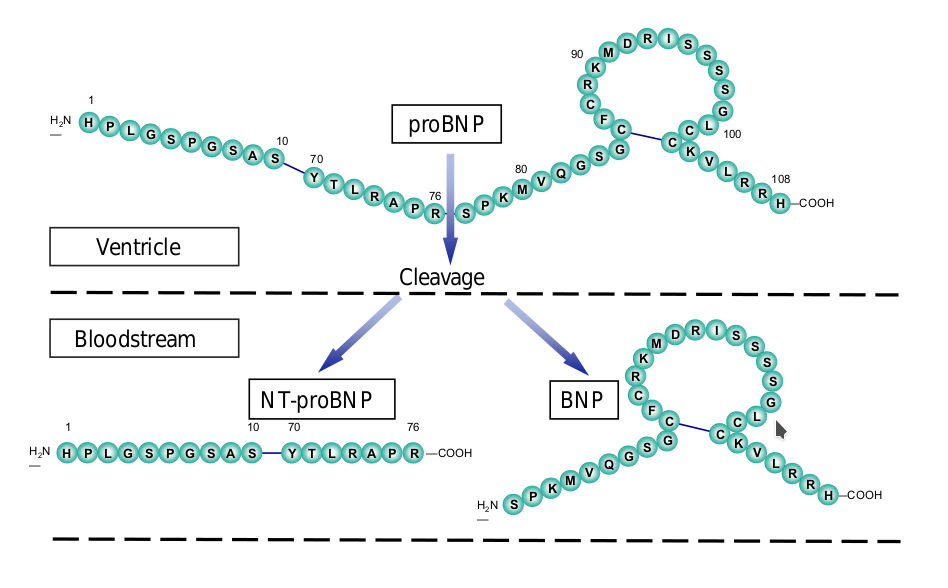
\includegraphics[scale=0.4]{../../images/BNP_secretion.png}
    \small\caption{Secretion of BNP and NtproBNP}
    \label{BNP_secretion}
\end{figure}

\subsubsection{BNP and NT-proBNP in clinical practice}
BNP and NT-proBNP plasma levels are promising tools in the daily management of suspected or established HF. Most studies on the use of BNP and NT-proBNP in clinical practice addressed their diagnostic properties. However, an increasing amount of evidence is available on the prognostic value of BNP and NT-proBNP and some studies provided hopeful results for the benefits of NT-proBNP guided medical treatment.

\textbf{Diagnosis}

Recent trials provided strong evidence that BNP and NT-proBNP are powerful diagnostic tools in exclusion and diagnosis of HF. The Breathing Not Properly study showed, by means of receiver operating characteristics analyses, that a BNP value of 100 pg/ml was the optimal value to differentiate patients with dyspnoea caused by HF from patients with dyspnoea due to pulmonary pathology at the emergency department Fig. \ref{BNP_ER}. \citep{Maisel2002}.  This value of 100 pg/ml also discriminated non-systolic HF (LVEF <45\%) from non-HF patients at the emergency department. It has also been suggested that BNP could be used to discriminate systolic from diastolic HF. Although non-systolic HF patients had significantly lower BNP plasma levels than systolic HF patients (LVEF >45\%), BNP only had modest added value in differentiating non-systolic from systolic HF. In another study, a BNP value of 100 pg/ml added significant value to the diagnosis of HF on top of clinical judgement. \citep{McCullough2002}

 An international pooled analysis of 1256 patients provided cut off values for NT-proBNP in an emergency department setting. An age independent cut point of 300 pg/ml had a negative predictive value of 98\%.  Additionally, an optimal strategy to identify acute HF was to use age stratified cut off points of 450, 900 and 1800 pg/ml for ages <50, 50-75, and >75 respectively which yielded 90\% sensitivity and 84\% specificity for acute HF Fig. \ref{NTBNP_ER}. \citep{Januzzi2006,Januzzi2005} Furthermore, BNP and NT-proBNP seem useful as diagnostic tools in primary care (where most patients with suspected HF are encountered and where only limited diagnostic tools are available) and as such are recommended in recent guidelines. \citep{Swedberg2005}

 The added value of these natriuretic peptides on top of established diagnostic tools, including symptoms and signs, has not been properly studied, in particular in relevant subgroups, and currently large studies are underway addressing this issue.  %CHECK
  Discharge diagnoses have been instrumental in providing estimates and time trends in prevalence and incidence of HF. However, previous studies in the Netherlands, Sweden and in the United States showed that respectively 20\%, 18\% and 33\% of the patients that were given the discharge diagnosis ‘HF’ at close examination did not have HF at all. \citep{Ingelsson2005,Goff2000} It is unknown whether the established BNP cut off value of 100 pg/ml can also be used at discharge after admission for HF.

\begin{figure}
    \centering
    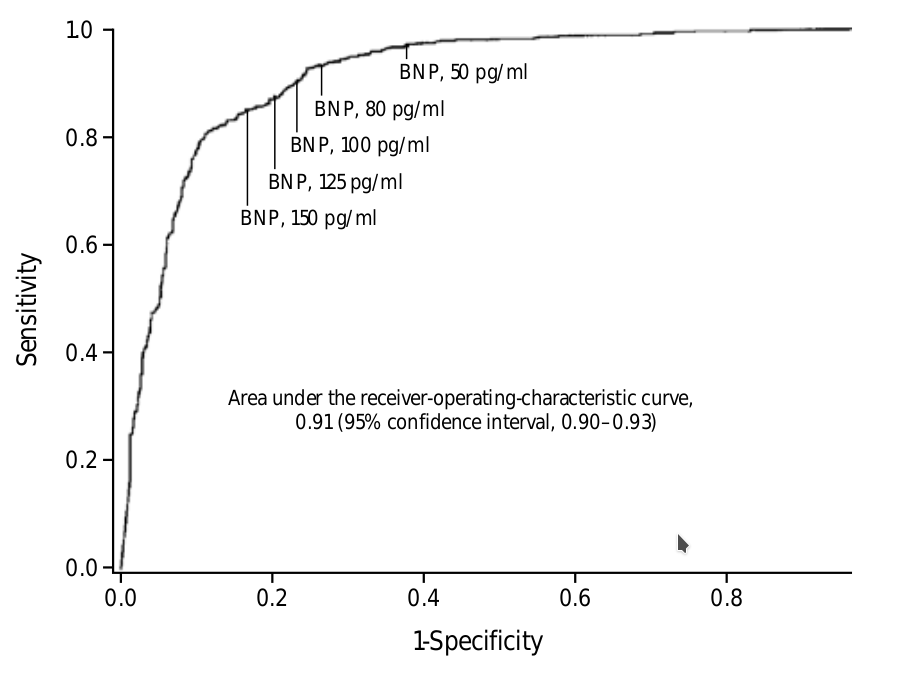
\includegraphics[scale=0.4]{../../images/BNP_ER.png}
    \small\caption{ROC curves for BNP in the diagnosis of heart failure at the emergency department.}
    \label{BNP_ER}
\end{figure}

\begin{figure}
    \centering
    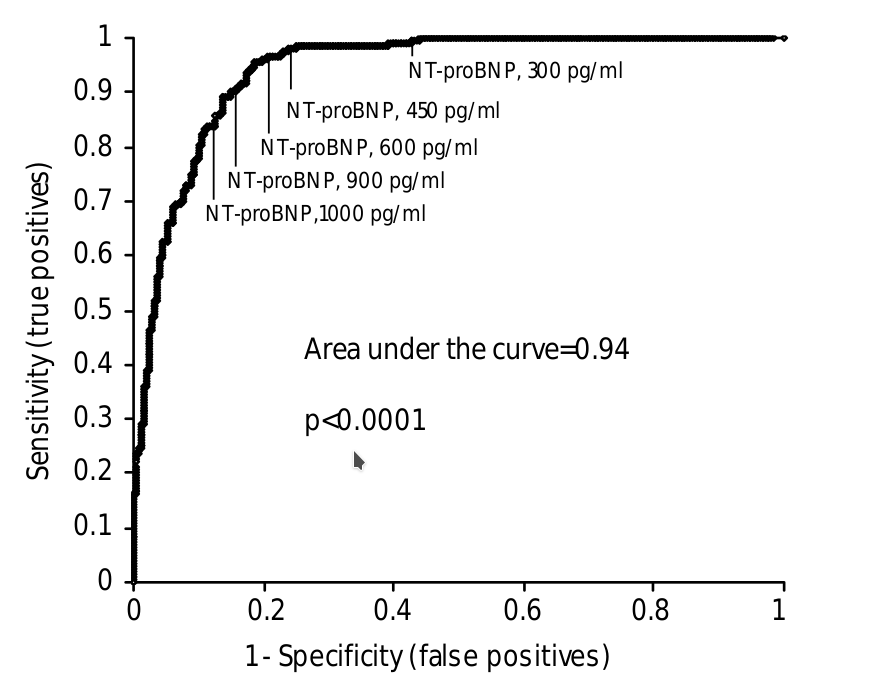
\includegraphics[scale=0.4]{../../images/NTBNP_ER.png}
    \small\caption{ROC curves for NTproBNP in the diagnosis of heart failure at the emergency department.}
    \label{NTBNP_ER}
\end{figure}


\textbf{Prognosis}

The prognostic value of BNP and NT-proBNP is well established in several groups of patients. An early study on 85 patients with chronic HF revealed that BNP is a strong independent predictor of mortality. \citep{Tsutamoto1997} Another study confirmed these results in a larger research population of 452 systolic HF patients (LVEF <35\%). In this study BNP was found to be a strong independent predictor of sudden death during a follow up period of 3 years. \citep{Berger2002}
Furthermore, NT-proBNP was a predictor of sudden death in this study population. A substudy of the COPERNICUS trial (n=1011) revealed that NT-proBNP was consistently associated with an increased risk for all-cause mortality and hospitalisation for HF in patients with severe HF (LVEF <25\%). \citep{Hartmann2004} Another study on 142 patients with advanced HF also reported that NT-proBNP was an independent predictor of all cause mortality. \citep{Gardner2003b}


\textbf{Guidance of treatment}

BNP and NT-proBNP are influenced by drugs that are prescribed to HF patients like diuretics, \citep{Tsutamoto2004} beta blockers, \citep{Richards1999} ACE inhibitors or angiotensine II receptor blockers \citep{Latini2002} and therefore these natriuretic peptides could possibly be used to guide medical treatment. A small study by the Australia-New Zealand Heart Failure Group including 69 patients with symptomatic HF provided evidence of the possible benefit of a NT-proBNP guided approach to therapy. Half of the patients received therapy guided by plasma NT-proBNP, therapy in the remaining patients was guided by clinical monitoring at the same frequency, but with the physician blinded to the NT-proBNP result. Clinical monitoring was based on scores assigned to 10 symptoms or signs of HF used in the Framingham criteria for HF.
The study found significantly lower mortality, fewer hospitalisations and episodes of decompensated HF in the NT-proBNP-guided therapy group (target 1680 pg/ml). \citep{Troughton2000} Larger studies are underway that are about to provide firmer evidence as to whether or not BNP and NT-proBNP can be used as a marker in the monitoring of treatment of HF patients. \citep{Buckley1999} %CHECK

\subsubsection{Variables influencing BNP and NT-proBNP levels: potential limitations?}
Although natriuretic peptide levels are of value in the diagnosis and prognosis of HF patients, several clinical conditions other than HF influence BNP and NT-proBNP plasma levels as well. These influences may be a disadvantage for the use of BNP and NT-proBNP in clinical practice of HF since it may lead to biased interpretations of the test results.

Cardiac variables:
BNP and NT-proBNP are also elevated in patients with acute coronary syndrome. After acute myocardial infarction, levels of BNP rise rapidly during the first 24 hours and then tend to stabilize, \citep{deLemos2001} and in patients with a Q-wave infarction, a peak in NT-proBNP levels was found after 12-48 hours. \citep{Talwar2000} In patients with unstable angina pectoris, BNP levels were found to be four times higher compared to patients with stable angina pectoris. \citep{Kikuta1996}
Moreover, atrial fibrillation resulted in increased BNP levels in patients without, but not in patients with HF. \citep{Knudsen2005} Right ventricular failure due to acute pulmonary embolism can also be determined by BNP. \citep{Tulevski2002} Furthermore, hypertensive patients have higher BNP and NT-proBNP levels compared to non-hypertensive subjects. \citep{Boomsma2001}

Non-cardiac variables:
A few studies in relatively small study populations without HF showed that anaemia causes elevated BNP levels \citep{Tsuji2004,Willis2005,Wold2005} and in a study on a small group of HF patients anaemia was also related to increased NT-proBNP levels. \citep{Wu2005}
However, besides that these studies were limited in sample size, they only investigated one of the two peptides and the effect of anaemia on NT-proBNP was investigated in HF patients only.
Furthermore, anaemia is often caused by renal dysfunction, but this co-morbidity has not been investigated in detail in these studies. Since both BNP and NT-proBNP are known to be elevated in case of renal dysfunction, \citep{Luchner2005} and because renal function and HF are interrelated, a study investigating the effect of anaemia and renal function on both BNP and NT-proBNP in HF patients is needed.
An additional variable that is related to both BNP and NT-proBNP is obesity. In several large studies lower natriuretic peptide levels were associated with higher body mass indexes. \citep{Das2005,Krauser2005,Mehra2004,Wang2004b} As far as diabetes is concerned, results are conflicting between BNP and NT-proBNP; BNP levels did not differ between patients with or without diabetes, \citep{Wu2004} but NT-proBNP levels seem to be higher in diabetic patients compared to non diabetics. \citep{Magnusson2004}
Furthermore, ascitic cirrhosis, hyperaldosteronism, hypercortisolism, carcinoma, subarachnoid hemorrhage, \citep{Pfister2004} lung cancer, tuberculosis and pulmonary embolism \citep{7} are clinical conditions with reported elevated natriuretic peptide levels.

Patient related variables:
Studies showed that both BNP and NT-proBNP levels are influenced by biological variation, with the biological variation of BNP being higher compared to NT-proBNP (up to 44\% and up to 35\% respectively). \citep{Bruins2004,Wu2003b}
Both BNP and NT-proBNP increase with advancing age and are higher in females compared to males in healthy subjects. \citep{Raymond2003} %Nevertheless it is unknown whether there are differences in the age and gender dependency between the two peptides and only limited data are available on the age dependency of BNP and NT-proBNP in HF patients. Furthermore, before BNP and NT-proBNP were discovered, Atrial Natriuretic Peptide (ANP) and N-terminal ANP (NT-ANP), natriuretic peptides that are mainly produced in the atria and with properties comparable to BNP and NT-proBNP, were studied. Although evidence is available on the superiority of BNP over ANP in the diagnosis of HF and of BNP/ NT-proBNP over ANP/ NT-ANP in the prognosis after myocardial infarction, it is unknown which peptide is influenced most by age and gender.

Previous research shows that BNP is related to maximal exercise performance. \citep{Kruger2002} Moreover, the influence of moderate physical activity (75\% of the maximum) on BNP levels was investigated in 10 healthy subjects, 10 HF patients with NYHA class I-II and in 10 HF patients with NYHA class III-IV. A significant increase in BNP levels was observed directly after exercise. \citep{McNairy2002} However, it is not known whether B-type natriuretic peptide levels also reflect sub-maximal functional capacity during daily activities and whether they are related to quality of life.


% \subsection{Coronary Artery Disease}
% An extremely short chapter.  No time to be wasted on it.
%
% \subsection{Coronary Artery Bypass Grafting}
% Also short
% \subsubsection{on-pump vs OPCAB}


\section{Clinical Considerations and Applications in Cardiac Diseases}
\subsection{ Circulating Levels of Cardiac Natriuretic Hormones}
\subsubsection{Physiological Considerations and Clinical Interpretation}
\subsubsection{ Influence of Age and Gender}
The circulating levels of CNH are regulated or modified by several physiological factors
(such as circadian variations, age, gender, exercise, body posture, and water immersion),
eating habits (especially sodium intake), clinical conditions (Table 5.1), and drugs (including corticosteroids, sex steroid hormones, thyroid hormones, diuretics, angiotensin-converting enzyme [ACE] inhibitors, and adrenergic agonists and antagonists) \citep{bib31} \citep{bib32} \citep{bib33} \citep{bib34} \citep{bib35} \citep{bib36}.

The wide variations of circulating levels of CNH in adult healthy subjects in relation to aging and gender could have a particular clinical relevance \citep{bib37} \citep{bib38} \citep{bib39} \citep{bib310} (Figs. 5.1 and 5.2, Table 5.2). Indeed, Vasan et al. \citep{bib39} demonstrated that the diagnostic accuracy of CNH assay for community screening is gender-dependent.

In order to explain these variations, the possible influence of sex steroid hormones on the CNH system, as well as the modification of the cardiovascular system with aging, should be taken into account \citep{bib311} \citep{bib312} \citep{bib313} \citep{bib314}. According to these mechanisms, the higher CNH values of women during the fertile adult period could be explained by the physiological stimulation of female sex steroid hormones. In particular, the BNP concentration is on average 36\% higher in women than in men aged less than 50 years \citep{bib37} (Figs. 5.1 and 5.2, Table 5.2). The increase in CNH with aging may be due to the decline in myocardial function and other organs (including kidney), typical of senescence \citep{bib315}. In this case, the CNH assay may be considered as a biochemical marker of increased risk of cardiac morbidity in old age \citep{bib316}. Moreover, the increase in CNH with aging may be due to a decrease in their clearance rate. Indeed, an age modulation of maximum binding capacity of clearance (C-type) receptors for CNH was reported in platelets of elderly persons \citep{bib317}.


%\subsubsection{ Comparison between the CNH Assay and that of CNH-Related Pro-Hormone Peptides}

All CNH derive from pre-pro-hormones (i.e., preproANP and preproBNP), containing a signal peptide sequence at the amino-terminal end. The pro-hormones (i.e., proANP and proBNP) are produced by cleavage of signal peptide, and then are further split into inactive longer NH-2 -terminal fragments (i.e., NT-proANP or NT proBNP), and a biologically active shorter COOH-terminal peptide (i.e., ANP or BNP), which are secreted in the blood in equimolar amounts (Figs. 3.11 and 3.12). However, ANP and BNP have a shorter plasma half-life and consequently lower plasma concentration, compared to NT-proANP and NT-proBNP (Table 4.1) \citep{bib31} \citep{bib32} \citep{bib33} \citep{bib34} \citep{bib35} \citep{bib36} \citep{bib37} \citep{bib318}.

Studies on structure-activity relationships have shown the importance for the binding to the specific receptors of the central ring structure of CNH, formed by a disulfide bridge between the two cysteine  residues. For this reason, only ANP and BNP, which present the disulfide bridge in the peptide chain, share the typical hormonal activity of CNH, while the NT-proANP and NT-proBNP do not \citep{bib31} \citep{bib32} \citep{bib33} \citep{bib34} \citep{bib35} \citep{bib36} \citep{bib37}.

Theoretically, setting up an immunoassay for NT-proANP and NT-proBNP should be easier because their plasma concentrations are higher than ANP and BNP \citep{bib318}.  On the other hand, NT-proANP and NT-proBNP immunoassays may be affected by several analytical problems, mainly concerning the different assay specificities; consequently, very different results are produced by different methods with a large bias \citep{bib32} \citep{bib35} \citep{bib36} \citep{bib318} (Table 4.1). The different analytical performance might affect the diagnostic accuracy of the assays, in discriminating between subjects with or without cardiac disease \citep{bib32} \citep{bib35} \citep{bib36}.

The respective advantages of measuring biologically active peptide hormones (ANP and BNP), or inactive peptides (NT-proANP and NT-proBNP) are summarized in Table. The assay of the inactive propeptides better fits the definition of disease marker than the assay of circulating levels of ANP or BNP, which, on the other hand, may be considered a more reliable index of the activation status of the CNH system. Considering the biochemical and physiological characteristics of the different peptides, it is conceivable that ANP is a better marker of acute overload and/or rapid cardiovascular hemodynamic changes than BNP and, especially, than NT-proANP or NT-proBNP \citep{bib32} \citep{bib35}. For example, circulating levels of ANP are known to be more affected by body position and decreased to a greater extent by a hemodialysis session in patients with chronic renal failure than those of BNP, while plasma NT-proANP is unchanged \citep{bib322}.% Furthermore, ANP increases more than NT-proANP during rapid ventricular pacing \citep{bib323}.

\subsubsection{ Resistance to the Biological Action of CNH}

% Deficiencies in the activity of the CNH system could explain altered electrolyte and fluid homeostasis occurring in chronic heart failure (HF) \citep{bib327} \citep{bib325} \citep{bib333}. However, the hypothesis proposing HF as a syndrome of CNH deficiency was challenged when the CNH system was more carefully investigated in experimental animals and humans \citep{bib327} \citep{bib325} \citep{bib333}.

Patients with chronic HF show increased CNH plasma levels compared to normal subjects (Table 3.1, Fig. 3.13). These findings have been defined the “endocrine paradox” in HF \citep{bib36}, i.e., extremely high circulating levels of hormones with powerful natriuretic activity in patients with congestive HF, who show physical signs of fluid retention and vasoconstriction due to a relatively poor biological activity of the CNH system. A blunted natriuretic response after pharmacological doses of ANP and BNP has been observed in experimental models and in patients with chronic HF, suggesting a resistance to the biological effects of CNH, principally natriuresis \citep{bib327} \citep{bib325} \citep{bib333} \citep{bib327} \citep{bib328} \citep{bib329} \citep{bib330} \citep{bib331}. This resistance syndrome was also demonstrated by in vivo turnover studies using radioactive tracers in patients with HF \citep{bib332} \citep{bib333}.

Resistance to the biological action of CNH could, theoretically, have three different causes (Table 5.3). First, circulating CNH could be, at least in part, inactive. Furthermore, a great fraction of CNH could be inactivated by plasma and tissue proteases before they bind to specific receptors. These two conditions account for all possible mechanisms acting at the pre-receptor level. Second, down-regulation of specific receptors could explain a reduced CNH activity. Finally, some mechanisms can act at postreceptor level, counteracting the biological effects of CNH.

% Mechanisms acting at pre-receptor level: Some peptides, derived in vivo or in vitro from degradation of intact proBNP, are biologically inactive, although they can be measured by immunoassay methods \citep{bib35} \citep{bib36} \citep{bib318}. Since the circulating levels of intact proBNP and of its derived peptides increase progressively with severity of HF, immunoassay methods can greatly overestimate the true biological activity of CNH in patients with severe HF \citep{bib36}. Unfortunately, at present, it is not possible to estimate the inaccuracy of CNH immunoassays because these methods use different, not standardized antibodies and calibrators, leading to highly different clinical results \citep{bib35} \citep{bib36} \citep{bib318} \citep{bib3131} \citep{bib335}.

A resistance to the biological action of CNH may be theoretically due to an increase in degradation (turnover) of circulating biologically active peptides. CNH are degraded in vivo and in vitro by several types of proteolytic enzymes, including serin-proteases, peptidyl arginine aldehyde proteases, kallikrein like proteases, and neutral endopeptidases (NEP) \citep{bib35} \citep{bib36} \citep{bib318} \citep{bib3131} \citep{bib335} \citep{bib336} \citep{bib337} \citep{bib338}.

Individual differences in the ability of heart tissue to mature the precursor of CNH peptides, or of peripheral tissues to degrade them, may help to explain why there are some differences in the clinical presentation among patients with HF with similar clinical severity and ventricular function \citep{bib36}.However,further studies are necessary to confirm this hypothesis.From a clinical point of view,it is important to note that some drugs sharing an inhibitory action on both NEP and ACE (so called vasopeptidase inhibitors) may have some beneficial effects in patients with arterial hypertension and/or HF because the administration of these durgs can potentiate the biological activity of CNH system by increasing the concentration of biologically active peptides \citep{bib339} \citep{bib340} \citep{bib341} \citep{bib342}.

It is important to note that renal function can affect the biological action of CNH in different ways .CNH are small peptides freely filtrated by renal glomerulus; the kidneys are probably responsible for about 50\% of metabolic clerance rate of plasma ANP and BNP and in this way renal diseases can affect the circulating levels of CNH.  Indeed,a decreased renal function greatly increases the plasma CNH concentration and consequently more peptide hormones are available for other target tissues (such as brain,vascular tissue,adrenal gland and so on) \citep{bib35}.However,luminal perfusion with ANP has been shown to reduce sodium efflux from the inner medullar collecting duct, suggesting that this hormone has also luminal sites of action.  As a consequence, a reduction in the filtration can potentially induce renal hypo-responsiveness to CNH. To date, however,ANP has been detected only on tubular basolateral membranes \citep{bib325}. %Thus, the mechanisms of CNH luminal action need to be elucidated before conclusions are drawn about the functional significance of reduced natriuretic peptide filtrations in the renal hypo-responsiveness to ANP and other natriuretic peptides.Finally,a resistance to the biological action of CNH may be theoretically also due to an increased renal filtration (clearance) of active peptides; at this moment, however, there are no consistent data to confirm this hypothesis.

Some studies suggest that the resistance to biological effects of CNH in HF may be due,in part,to variations in the relative amount of the three different types of natriuretic peptide-specific receptors.In particular,there could be an upregulation of type C receptors (NPR-C) with a parallel down regulation of type A and B receptors (NPR-A and NPR-B) \citep{bib343} \citep{bib344} \citep{bib345} \citep{bib346} \citep{bib347}. NPR-A and NPR-B mediate all known hormonal actions of CNH, therefore their down-regulation should induce a deactivation of the CNH system. The upregulation of NPR-C receptors that strongly contribute to the clearance of biologically active peptides could further increase the resistance to CNH in patients with HF \citep{bib343}.

These findings are well in accordance with the results of in vivo kinetic studies obtained using radioactive tracers in patients with HF \citep{bib332} \citep{bib333}. Moreover, a  study confirmed that mRNA expression levels of ANP, BNP and the NPR-C receptor were markedly increased in human failing hearts \citep{bib346}. Reversal of cardiomyocyte hypertrophy during left ventricular assist device support was accompanied by normalization of ANP, BNP and NPR-C mRNA levels and a significant recovery of responsiveness to ANP \citep{bib347}.  However,  \citep{bib348} found that neither NPR-A nor NPR-B were internalized or degraded in response tonatriuretic peptide binding in %293T
cultured cells.

Another well-characterized deactivation mechanism is the process by which an activated receptor is turned off, commonly referred to as “desensitization”. Phosphorylation of the intracellular kinase homology domain of NRP-A and NPR-B is required for hormone-dependent activation of the receptor, while dephosphorylation at this site causes desensitization. Deactivation of the CNH system via desensitization of NRP-A and NPR-B can occur in response to various pathophysiological stimuli \citep{bib348} \citep{bib349} \citep{bib350} .

% Further studies are necessary to clarify what is the most important mechanism of deactivation of CNH system acting in vivo at receptor level in patients with heart failure: the down-regulation (of NPR-A and NPR-B), the upregulation (of NPR-C), or the desensitization (of NPR-A and NPR-B).

A peripheral resistance to the biological effects of CNH may play an important role in other clinical conditions, besides HF. For example, NPR-C is also present on cellular membranes of adipose tissue. It was suggested that the increase in NPR-C receptors observed in obese subjects can in turn increase the peripheral degradation of CNH and consequently blunt the action of the CNH system \citep{bib351} \citep{bib352}. Indeed, studies have documented decreased circulating levels of CNH (especially BNP) in obese subjects, compared to nonobese subjects matched for age and gender \citep{bib351} \citep{bib354}. This reduced activity of the CNH system may increase the risk of developing arterial hypertension and other cardiovascular diseases due to the non-contrasted and therefore prevailing effects of the counter regulatory system with sodium-retentive and vasoconstrictive properties \citep{bib352} \citep{bib353} \citep{bib354}

However, studies found that the NPR-C receptor could be coupled to a G-protein that inhibits cyclic AMP synthesis. These receptors, which are present in great amount especially on the endothelial cell wall, may mediate some paracrine effects of CNP on vascular tissue \citep{bib355} \citep{bib356} \citep{bib357}. Therefore, further studies will be necessary to elucidate the possible role of NPR-C receptors as modulators of CNH action and/or degradation in peripheral tissues.

A large number of studies demonstrated that the activation of the neuro-hormonal system accelerates the left ventricular functional impairment in patients with HF \citep{bib31} \citep{bib32} \citep{bib33} \citep{bib34} \citep{bib35} \citep{bib36} \citep{bib358} \citep{bib359} \citep{bib360}. Drugs that contrast the detrimental effects of the neuro-hormonal system activation play a key role for the current pharmacological treatment of HF. Some of these, such as ACE inhibitors, angiotensin II receptor blockers, $\beta$-blockers, and spironolactone decrease the circulating levels of CNH \citep{bib35} \citep{bib361} \citep{bib362} \citep{bib363} \citep{bib364} \citep{bib365},“normalize” their kinetics, and increase their biological activity. Furthermore, they enhance the natriuretic effect of ANP or BNP analogs administered to patients. In other words, the treatment with this type of pharmacological agents decreases the systemic resistance to the biological effects of CNH \citep{bib327} \citep{bib333}.

Patients with HF show a progressive and parallel increase in CNH levels and in some neuro-hormones and cytokines. This increase can be closely related to disease severity, as assessed by functional NYHA class (Table 3.1, Fig. 3.13). Plasma BNP values, normalized by mean values found in healthy subjects, are significantly higher than other normalized neuro-hormone and cytokine values in HF (Fig. 5.3, Table 5.4) \citep{bib360}.

On average, the response of the CNH system to the increasing challenge of disease severity may not be linear (Fig. 5.4). The curve reported in Figure 5.4 suggests that the CNH system responds with a sharp increase in BNP plasma concentration in the early phase of HF (NYHA class I-II patients), followed, with the clinical progression of the disease, by a blunted increase (NYHA class III), and finally by a plateau (NYHA class IV) (Table 3.1, Fig. 5.4). These findings are consistent with the results from in vivo kinetic studies, indicating that ANP turnover (i.e., metabolic clearance rate and production rate) and natriuresis are both increased in patients in the early phase of HF (NYHA class I), as compared to patients with congestive HF \citep{bib327} \citep{bib333}. This suggests that resistance to the biological action of CNH is characteristic only of the congestive stage of HF. During the asymptomatic, early phase of the disease, the CNH system is able to compensate for the overactivity of the counter regulatory system (Fig. 5.4).

% In conclusion, several mechanisms occurring at the pre-receptorial, receptorial and post-receptorial levels may play a role in inducing peripheral resistance to the biological effects of CNH in HF. However, the overwhelming activation of the counter-regulatory system should be considered the predominant pathophysiological mechanism. The data discussed so far also suggest that monitoring the degree of systemic resistance to the biological effects of CNH could be clinically useful in the follow-up of patients with HF.

\subsubsection{ Diagnostic Accuracy of CNH Assay in Plasma from Patients with Cardiac Diseases}

The CNH system activation is modulated not only by hemodynamic factors, but also by the activity of the counter-regulatory neuro-hormonal system.% The response of the CNH system to chronic pathophysiological stimuli may be log-like (Figs. 3.13 and 5.4).
Consequently, it is likely that very small changes in hemodynamics, not assessable by echocardiographic examination, may produce significant (and measurable) variations in plasma concentrations of CNH. Moreover, studies have indicated that very small changes in some neuro-hormones and cytokines can produce wider variations in BNP circulating levels \citep{bib360} (Fig. 5.3).

It is well known that changes in hemodynamic parameters (such as left ventricular ejection fraction, EF) and plasma CNH levels (expressed in a log scale) are closely related in patients with cardiovascular diseases (Fig. 5.5) \citep{bib32} \citep{bib33} \citep{bib34} \citep{bib35} \citep{bib319} \citep{bib358} \citep{bib359} \citep{bib360} \citep{bib361} \citep{bib362} \citep{bib363} \citep{bib364} \citep{bib365}. However, correlations between plasma CNH levels and echocardiographically measured parameters, such as left ventricular EF, myocardial mass and chamber volumes, are usually less close in the general population (large community-based sample, including healthy subjects with or without individuals with asymptomatic myocardial dysfunction) \citep{bib38} \citep{bib39} \citep{bib366} \citep{bib367}, as well shown dy data reported in Figure 5.6.

It should be emphasized that the recognition of HF syndrome is not equivalent to the clinical diagnosis of cardiomyopathy or to the assessment of left ventricular dysfunction, these latter terms describing possible structural reasons for the development of HF. Instead, HF is a clinical syndrome that is characterized by specific symptoms (namely dyspnea and fatigue) and signs (namely fluid retention). There is no diagnostic test for HF, because it is largely a clinical diagnosis based on a careful history and physical examination \citep{bib368}. Therefore, there are no objective criteria for the identification and/or clinical stratification of patients with suspected HF; several “reference (gold) standards” \citep{bib371}, based on clinical, laboratory and instrumental examinations, can be used to evaluate the diagnostic accuracy of the CNH assay. For this evaluation, some studies took into consideration only echocardiographic assessment of ventricular dysfunction, while in others either results of echocardiography or all clinical data have been used for the diagnosis of HF \citep{bib35}.

Unfortunately, using echocardiography as the unique reference standard may lead to misinterpretations when evaluating the diagnostic accuracy of the CNH assay. A systematic review of clinical studies in patient populations with a prevalence of HF ranging from 3.8\% to 51\% to determine the diagnostic accuracy of BNP assays found that the sensitivity (ranging from 90 to 97\%) was much less variable (by 4.4-fold) than the specificity (ranging from 53 to 84\%) \citep{bib35}.

Furthermore, in a meta-analysis \citep{bib372}, diagnostic accuracy of BNP assays greatly varied according not only to the group of patients studied, but also to the reference standard used (left ventricular EF <40\% or <55\%, diagnosis of diastolic dysfunction, diagnosis of systolic + diastolic dysfunction, or integrative clinical criteria). These data indicate that the choice of a suitable and accurate reference standard for evaluation of the diagnostic accuracy of the BNP assay in patients with HF may be a problem that is actually underestimated in the literature. For a proper definition of diagnostic accuracy, tested individuals should be grouped into those with and without disease, by means of an independent clinical judgment, considering both the CNH assay and echocardiographic data.

Careful echocardiographic examinations usually show slightly better or even similar diagnostic accuracy than the BNP assay in patients with cardiac diseases \citep{bib373} \citep{bib3178}. On the other hand, the CNH assay may have some advantages compared to echocardiographic examinations alone in specific clinical settings. For example, Williams et al. suggested that in patients with chronic HF, the NT-proBNP assay reflects functional cardiac impairment and decreased exercise capacity (measured by peak exercise oxygen consumption) better than the left ventricular EF \citep{bib375}.

Several studies indicate that BNP and NT-proBNP are powerful and independent risk markers of cardiovascular events (especially mortality) not only in patients with HF, but also in those with acute coronary syndrome, as reported in  and systematic reviews \citep{bib35} \citep{bib376} \citep{bib377} \citep{bib378}. Some studies also suggested that the cardiovascular risk increases progressively to CNH concentration \citep{bib377} \citep{bib378} \citep{bib3194}; that is, there is no threshold that actually identifies patients with null risk.


%VERY IMPORTANT
Diagnostic sensitivity of BNP/NT-proBNP assays in detecting left ventricular systolic dysfunction could be suboptimal in asymptomatic or low-risk individuals, especially in women \citep{bib39}. Specificity of BNPassays in patients with HF ranged from 53 to84\% and positive predictive values from 3 to 85\% inseveral studies. These data indicate that CNH assays can produce a relatively large number of false-positive results. Consequently, many individuals, actually without HF (about 15-60\% of those with positive CNH tests),mightundergo expensive and/or harmful investigations to rule out the disease, or even be inappropriately labeled as cardiac patients \citep{bib35}.

Several false-positive results can be observed in patients with various clinical diagnoses, as reported in Table 5.1. In these patients, increased plasma BNP may predict, even in the presence of a normal echocardiographic examination, an increased risk of mortality or major cardiac events, including pulmonary embolism \citep{bib380} \citep{bib381} \citep{bib382} and hypertension \citep{bib383}, renal failure \citep{bib384} \citep{bib385}, septic shock \citep{bib386}, some chronic inflammatory diseases (such as amyloidosis and sarcoidosis) \citep{bib387} \citep{bib388}, and diabetes mellitus \citep{bib389}.

On the other hand, false-negative results could be found in patients on treatment with anti-adrenergic agents, diuretics and/or ACE inhibitors, all drugs that can reduce CNH levels \citep{bib35}. As shown in Figure 5.7, a large number of patients with only mild HF (NYHA classes I and II) may have values slightly above or even under the 99th percentile of distribution values of BNP concentration in healthy subjects. In these patients, successful treatment and consequent improvement in cardiac function and exercise capacity, and reduction in filling pressure and cardiac volumes, is usually associated with a marked fall in CNH levels: thus, a larger number of patients could have BNP values within the reference range values \citep{bib35} \citep{bib390}.

However, at matched echocardiographic alterations, patients in whom BNP levels drop in response to therapy have a reduced rate of major cardiac events or mortality, compared to untreated hypertensive patients, who could have similar echocardiographic abnormalities. This represents the rationale for using the CNH assay for therapy decision making and for monitoring HF patients \citep{bib35} \citep{bib361} \citep{bib362} \citep{bib363} \citep{bib364} \citep{bib365}.

In populations with a higher prevalence of cardiac diseases, including only individuals with a clinical suspicion of HF, the diagnostic sensitivity of BNP can improve up to 95\%, or even more, as long as appropriate cut-off values are selected \citep{bib35} \citep{bib372}. In this case, a strategy called “SnNout”, which maximizes test sensitivity, could be used to rule out the presence of HF \citep{bib391}. Furthermore, CNH assay also shows high (>95\%) negative predictive values \citep{bib35} \citep{bib320}, which can help to confirm the absence of HF. This is the rationale for choosing the CNH assay as the first step for an algorithm for the diagnosis of HF \citep{bib369} \citep{bib370}. Such a clinical strategy has proved successful in some  studies evaluating the cost-effectiveness of using plasma BNP measurements for screening of cardiac dysfunction in the general population \citep{bib392} \citep{bib393} \citep{bib3171}.


\subsubsection{ Biological Variation of Plasma BNP: a Problem or a Clinical Resource?}

The variability of measured plasma concentrations of many substances is due to three different sources: pre-analytical, analytical and inherent biological variation. The latter is usually described as a random variation around a homeostatic setting point, and defined as the intra-individual or within-subject biological variation \citep{bib395}.

% Several physiological parameters and endogenous substances are closely regulated by complex biological mechanisms in such a way as to vary little. If a random variation is assumed for an analyte, the effect of imprecision on dispersion can be taken into consideration for setting generally applicable quality specifications for assay performance in order to indicate an acceptable (or desirable) degree of assay precision. Accordingly, the desirable assay imprecision should be equal to or less than half of the intra-individual biological variation \citep{bib396} \citep{bib397}.

In order to achieve a correct interpretation of serial test results that are collected for follow-up or tailored treatment of HF patients, several studies \citep{bib397} \citep{bib398} \citep{bib399} \citep{bib3100} \citep{bib3101} evaluated the biological variation of BNP and its related peptides, in both healthy subjects and cardiac patients. Due to secretory bursts and its rapid turnover (half-life about 15-20 min) \citep{bib31} \citep{bib3102} , it is not surprising that intra-individual biological variations of plasma BNP levels were found to be very large, in both healthy subjects and patients with heart failure (ranging from 30 to 50\%) \citep{bib397} \citep{bib399} \citep{bib3100} \citep{bib3101}.  %Assuming a random variation around a homeostatic setting point, the calculated reference change values at 95\% confidence interval ranged from 99 to 130\% for BNP in healthy subjects and patients \citep{bib397} \citep{bib399} \citep{bib3100} \citep{bib3101}.
According to this, only a decrease of more than 50\% or a more than 2-fold increase in plasma BNP should be assumed to be statistically significant in an individual patient.

In contrast with this assumption, a clinical trial \citep{bib390} has suggested that a BNP decrease inferior to this calculated reference change could be clinically relevant in patients with heart failure. In this study, only the group of patients treated with the \beta-blocker agent carvedilol, who respond on average with a decrease of only 38\% in plasma BNP, showed a clinical improvement \citep{bib390}.

Furthermore, several studies have demonstrated that cardiovascular risk (mortality or major cardiovascular events) increases continuously and progressively throughout the whole range of BNP concentrations in patients with cardiovascular diseases \citep{bib35} \citep{bib377} \citep{bib378} \citep{bib3194}.

In order to explain these conflicting findings, it should be taken into account that BNP secretion is closely regulated by specific pathophysiological mechanisms. Thus, changes in plasma hormone levels cannot be interpreted as random variations around a setting point, but as strictly determined by the activation level of the counter-regulatory system and by changes in hemodynamics. The clinician should look at the intra-individual variation in BNP as a mirror of variation in neuro-endocrine network activity. According to this hypothesis, it was suggested to consider all changes in BNP concentration as potentially clinically relevant, even when narrower than the calculated intra-individual biological variation \citep{bib3103}.
In other words, BNP variations should be interpreted and considered by physicians, as the variability of heart rhythm and blood pressure, by taking into account clinical history and examination, comprehensive of the response to specific treatments, as well as of laboratory and instrumental test findings.

% There is another important practical consequence of this approach. According to an intra-individual biological variation of about 30\%, the estimated imprecision goal for BNP immunoassays should be 15\% (i.e., equal to half of the intra-individual variation) \citep{bib395} \citep{bib396}. On the contrary, we suggest that all the measured variations of plasma BNP greater than two to three times the analytical imprecision of assay used should be potentially considered as clinically relevant. Following this approach, the assay imprecision of BNP immunoassays should be as low as possible. Of course, the great number of pathophysiological mechanisms affecting the CNH system makes it sometimes difficult for clinicians to recognize the cause(s) of variations in its activity. However, we believe that the BNP assay should be considered as an intellectual spur for the search for an explanation of variations in hormone concentrations, which should always be related to pathophysiological stimuli and/or pharmacological interventions. In this sense, the assessment of BNP time-course concentrations is a novel, meaningful diagnostic tool for the follow-up of patients with cardiac disease.

\subsection{ CNH Assay as Diagnostic and Prognostic Tool in Cardiac Diseases}
In this second part of the Chapter 5, we will review the clinical relevance of CNH assay
(especially of BNP and NT-proBNP). There has been an explosion of clinical researches and trials concerning the routinary use of CNH (especially BNP) assay in the diagnosis and risk stratification of patients with cardiovascular diseases in the first years of
the new century . It is clearly impossible to cover all these scientific contributes. In order to reduce the number of references
without reducing the efficacy and objectiveness, we have used systematic reviews and
meta-analyses, when available.
First, we will review the clinical relevance of CNH assay in the screening and classification of patients with cardiac dysfunction, divided according to the severity of disesae and age, or associated to some particular clinical conditions (such as myocardial
infarction or treatment with cardiotoxic drugs) . Moreover, we will discuss the diagnostic accuracy and clinical relevance of assay in coronary artery disease , where more  BNP and NT-proBNP are increasingly frequently assayed with (almost in part) unexpected results. Finally, the diagnostic accuracy of CNH assay will be compared to that of other clinical tests, such as ECG,
echocardiogram and chest radiogram .
The last part of the Chapter is dedicated to prognostic relevance of CNH assay in
cardiac diseases and general population , to relevance of
measurement of CNH in tailoring the therapy , and to its cost-effectiveness  in patients with HF.

\subsubsection{ Use of CNH Assay in the Screening and Classification of Patients with Cardiac Dysfunction}

The diagnosis of HF can often be difficult, mainly in primary care settings, where patients may present with non-specific symptoms and signs, such as dyspnea, fatigue, and ankle swelling \citep{bib368} \citep{bib369} \citep{bib370}. In several population-based studies, fewer than 40\% of patients with a suspected diagnosis of HF in primary care had this diagnosis confirmed by more specific and accurate clinical investigations, which are often expensive, timeconsuming and demanding for the patient \citep{bib368} \citep{bib369} \citep{bib370} \citep{bib3104} \citep{bib3105}. As a result, a relatively simple and inexpensive biochemical test (such as the CNH assay) may be very useful to confirm the clinical suspicion of HF in this clinical setting \citep{bib35} \citep{bib3131} \citep{bib335}.

\subsubsection{ Diagnostic Accuracy of CNH Assay in Asymptomatic,}
\strong{Mild Ventricular Systolic Dysfunction}

Patients with asymptomatic left ventricular systolic dysfunction are likely to have lower plasma BNP than those with overt HF \citep{bib32} \citep{bib33} \citep{bib34} \citep{bib35} \citep{bib3131} \citep{bib335} \citep{bib362} \citep{bib363} \citep{bib364} \citep{bib365} \citep{bib366} \citep{bib372}, as shown in (Fig. 3.13.)

Two large studies \citep{bib39} \citep{bib366} evaluated the diagnostic accuracy of the CNH assay as a screening method in a general population. The first study analyzed the Framingham Heart Study cohort (3,177 individuals) using BNP and NT-proANP in the evaluation of left ventricular hypertrophy and systolic dysfunction in a community population \citep{bib39}.

The presence of the disease was evaluated by using echocardiographic findings (the prevalence of left ventricular systolic dysfunction was 9.3\% in the 1,470 men and 2.5\% in the 1,707 women tested, respectively). The area under the curve (AUC) of receiver operating characteristic (ROC) analysis for CNH assay for identifying both left ventricular hypertrophy and systolic dysfunction was on average about 0.75, with a good specificity (assumed 95\% both for men and women) and negative predictive value (NPV, on average ranging from 92\% to 97\% in men, and from 91\% to 98\% in women), but a poor sensitivity (i.e., ranging from 27\% to 28\% in men, and from 13\% to 40\% in women) and positive predictive value (PPV, from 22\% to 38\% in men, and from 5\% to 40\% in women), using gender-related BNP cut-off values \citep{bib39}.

The aim of the second study was to examine the validity of plasma BNP measurement for detection of various cardiac abnormalities in a rural Japanese population (1,098 subjects, 693 men and 405 women), with a low prevalence of coronary heart disease and left ventricular systolic dysfunction (i.e., only 37 participants, corresponding to 3.0\%, showed an EF <30\%). The diagnosis was carried out by two independent cardiologists based on a medical questionnaire, chest radiogram, electrocardiogram (ECG), and echocardiographic report. The optimal threshold for identification of disease was a BNP concentration of 50 ng/l (14.4 pmol/l), with an area under the ROC curve of 0.970, a sensitivity of 89.7\%, a specificity of 95.7\%, PPV of 44.3\%, and NPV of 99.6\%, respectively. \citep{bib366}

The conclusions of these two studies, though similar in aim, as well as in clinical and experimental protocols, were strongly conflicting. The Japanese study suggested that the BNP assay is a very efficient and cost-effective mass screening technique for identifying patients with various cardiac abnormalities regardless of etiology and degree of left ventricular systolic dysfunction \citep{bib366}, while the Framingham study suggested only limited usefulness of the CNH assay as a mass screening tool for this clinical condition, especially in women \citep{bib39}.

This discrepancy may be due to the different gold standard used for the diagnosis of heart failure adopted in the two studies, as discussed in a previous paragraph . However, these two studies, taken as a whole, indicate that the CNH assay may have only a limited usefulness as a screening method for HF in a general population, owing to the poor sensitivity and PPV. However, both studies also found good specificity and NPV, thus suggesting that the CNH assay may be used to rule out HF in an asymptomatic individual.

\subsubsection{ Diagnostic Accuracy of CNH Assay in Patients with Suspected HF}

Many studies \citep{bib392} \citep{bib3108} \citep{bib3109} \citep{bib3110} \citep{bib3111} \citep{bib3112} \citep{bib3113} \citep{bib3114} \citep{bib3115} \citep{bib3116} \citep{bib3117} \citep{bib3118} \citep{bib3119} \citep{bib3120} \citep{bib3121} \citep{bib3121} \citep{bib3123} \citep{bib3124} \citep{bib3125} \citep{bib3126} \citep{bib3152} \citep{bib3128} have suggested that the CNH assay could be useful as a screening method and/or for the differential diagnosis in patients suspected of HF in different clinical settings:
\begin{itemize}
  \item randomly selected high-risk community populations
  \item primary-care patients with a new diagnosis of HF
  \item patients with acute dyspnea in the emergency department
  \item consecutive unselected hospital inpatients
  \item patients admitted to the intensive care unit.
\end{itemize}

The studies concerning the diagnostic accuracy of the CNH assay in patients with HF have also been analyzed by two systematic reviews \citep{bib35} \citep{bib372}; unfortunately, these studies showed quite heterogeneous data, thus introducing some bias in the statistical analysis. In particular, even some high quality studies were not designed with the primary goal of evaluating the diagnostic accuracy of the CNH assay. Indeed, this aim was considered only at a post-hoc analysis and retrospectively assessed in blood samples collected for different original purposes, some years before the actual evaluation of diagnostic accuracy. This may introduce a significant bias, although its true clinical relevance is difficult to assess \citep{bib35}.

The second most important cause of heterogeneous data is the different reference (gold) standard used to evaluate the diagnostic accuracy of the CNH assay. In some studies, the patients studied were stratified and grouped according to clinical severity, as described by functional classification (usually NYHA classification). In other studies, only echocardiographic measurements were used as “gold standard” for the accuracy of the CNH assay for the diagnosis of left ventricular dysfunction (and not for the clinical diagnosis of HF) \citep{bib35} \citep{bib372}.

Furthermore, comparison of studies concerning the diagnostic accuracy of CNH assay is also difficult because different populations were enrolled and different immunoassays were used. Indeed, diagnostic accuracy (especially predictive values) is strictly dependent on disease prevalence (pre-test probability), which greatly varies according to the clinical setting considered (i.e., screening for general population, out-patients seen by a general practitioner, or in primary care, emergency department, coronary care unit, and so on). In particular, the prevalence of HF in the populations studied varied from less than 5\% (in studies of screening of asymptomatic population) to more than 50\% (in studies including patients referred to hospital with suspicion of HF) \citep{bib35}.

% Another factor, often underestimated, is that the “gold standard” (which is not an objective rule, but a clinical synthesis or another diagnostic test) could vary with the disease prevalence, sometimes in a different manner than the CNH assay.
Finally,  data reported in the literature suggested that diagnostic accuracy may vary significantly in relation with the specific cardiac peptide measured and/or immunoassay used.
% At the present time, the different BNP immunoassays also show greatly different imprecision \citep{bib3132}. Consequently, it is not clear whether the observed significant variation in diagnostic accuracy is due to a difference in pathophysiological behavior of measured peptides and/or in assay performance.
Unfortunately, some studies do not clearly indicate the type of immunoassay used to measure CNH, while the majority do not report the assay performance (and often even the reference values) evaluated in their own laboratory.\citep{bib35}

Taking all studies as a whole, a meta-analysis showed that the odds ratio for diagnostic accuracy of BNP assay in different groups of patients with suspected HF is highly significant. In particular, the pooled diagnostic odds ratio, when clinical criteria were used as gold standard for HF, was 30.9 (95\% confidence interval 27.0-35.4), while it fell to 11.9 (8.4-16.1) when a value $\leq$40\% of left ventricular EF, estimated by echocardiography, was used as reference standard \citep{bib372}.

% Diastolic dyfunction can play a major role in determining signs and symptoms in patients with congestive HF \citep{bib365} \citep{bib3120} \citep{bib3121}. Although Doppler echocardiography is currently used to examine the left ventricular diastolic filling dynamics, the limitations of this technique suggest the need for other objective measures \citep{bib3122}. Despite these limitations, several studies indicated that the CNH assay, in particular the BNP assay, may be useful for the diagnosis of left ventricular diastolic dysfunction \citep{bib3123} \citep{bib3125} \citep{bib3126}. However, some conflicting results have been reported, probably due to the different cause of and/or mechanisms responsible for cardiac dysfunction \citep{bib3152} \citep{bib3128}.

In a metaanalysis, including data of three studies comparing the diagnostic accuracy of BNP assay in patients with diastolic dysfunction, the pooled odds ratio was 28.3 (95\% confidence interval 2.66-300.5). However, a bias may affect these studies, as suggested by the significant test of heterogeneity \citep{bib372}.

Finally, \citep{bib3133} evaluated the effect of NT-proBNP assay on the clinical diagnostic accuracy of HF in primary care by means of a prospective, randomized controlled trial in 305 patients. Each patient was randomized in two groups, one in which the general practioner had at their disposal the NT-proBNP assay results (NT-proBNP assay group), while the other did not (control group). The diagnostic accuracy improved by 21\% in the NT-proBNP assay group and by 8\% in the control group (p = 0.002). This study indicates that NT-proBNP measurement significantly improves the clinical diagnostic accuracy of HF in general practice \citep{bib3133}.

\subsubsection{ Diagnostic Accuracy of CNH Assay in Patients with Acute Myocardial Infarction}

Circulating levels of CNH increase after acute myocardial infarction (AMI); the extent of the increase is related to the size of the infarct \citep{bib3134} \citep{bib3135} \citep{bib3136} \citep{bib3137}. Patients with smaller infarcts tend to have a monophasic increase in plasma BNP, peaking at 20 hours after the onset of symptoms; on the other hand, those with larger infarcts, lower EF, and clinical signs of HF may present a further peak at 5 days after admission \citep{bib3135}. Other studies are less convincing regarding the ability of the CNH assay to identify patients with significant myocardial dysfunction after AMI \citep{bib3138} \citep{bib3139}. These conflicting results could be due to the differences in sample collection time, type of CNH (ANP, BNP, or NT-proBNP) measured, type of assay, and inclusion criteria adopted. However, persisting elevation of CNH levels at 1 or 2 months after AMI usually suggests a high risk of adverse remodeling and subsequent HF \citep{bib35}.

The diagnostic accuracy of the BNP assay in patients with myocardial infarction was evaluated in a  meta analysis \citep{bib372} taking into account only two studies \citep{bib3140} \citep{bib3177}, fitting the inclusion criteria of this analysis; the pooled odds ratio was 9.4 (95\% confidence interval 4.5-19.4).

\subsubsection{ Diagnostic Accuracy of CNH Assay in Elderly People}

Heart failure is primarily a disease of old age; chronic HF increases in prevalence with aging from <1\% in people aged <65 years to >5\% in those >65 years of age, and this clinical condition is the first cause of morbidity and mortality in older people \citep{bib368} \citep{bib369} \citep{bib370} \citep{bib3193}. A  study demonstrated that elderly patients present with more advanced HF, as evidenced by their higher morbidity and mortality rate along with greater neurohormonal activation \citep{bib3193}. According to these findings, elderly people should be considered to be a population with high risk for developing HF and so the BNP/NT-proBNP assay may be useful as a screening test for HF in older age. Indeed, several studies reported that the BNP/NT-proBNP assay could be clinically useful in elderly people suspected to have HF \citep{bib316} \citep{bib3193} \citep{bib3143} \citep{bib3144} \citep{bib3145} \citep{bib3146} \citep{bib3147}.

Two studies compared the diagnostic accuracy of the BNP assay and that of ECG in elderly people screened for HF. A prospective cohort study specifically evaluated the diagnostic accuracy for HF of BNP assay in 299 consecutive patients (mean age 79 years, 65\% women) attending day-hospital over a period of 13 months. This study suggested that both BNP assay and ECG were sensitive in detecting left ventricular systolic dysfunction, but lacked specificity (but the combination of the two tests improved diagnostic accuracy) \citep{bib3143}.

The other study reported that both the ECG and the plasma concentration of BNP were highly efficient in excluding left ventricular systolic dysfunction in 407 75-year-old subjects. However, compared with the BNP, the ECG yields a lower number of false-positive cases. Therefore, this study suggested that in screening for left ventricular systolic dysfunction in elderly people, the BNP assay has a diagnostic value in addition to the ECG, but only in individuals with abnormal ECG \citep{bib3144}.

Another study indicated that the BNP assay may be particularly useful in ederly patients, especially in differentiating cardiogenic pulmonary edema from respiratory causes of dyspnea \citep{bib3146}. Screening of populations with more than 1\% prevalence of HF (such as people with age more than 60 years) with BNP followed by echocardiography should provide a health benefit at a cost that is comparable to or less than other accepted health interventions \citep{bib3145}. Finally, the NT-proBNP assay was demonstrated to be useful for detecting HF among people living in elderly nursing homes \citep{bib3147}.


\subsubsection{ Detection of Drug Cardiotoxicity by means of BNP Assay}

% Another example of the clinical relevance of BNP assay is the possibility of identifying HF caused by drug cardiotoxicity \citep{bib3148} \citep{bib3149} \citep{bib3150} \citep{bib3151} \citep{bib3152} \citep{bib3153}. Cardiotoxicity is a potential side-effect of some chemotherapeutic agents \citep{bib3154}. The anthracycline class of cytotoxic antibiotics are the most famous, but other chemotherapeutic agents can also cause serious cardiotoxicity and are not so well recognized (including cyclophosphamide and fluorouracil) \citep{bib3154}. In a large retrospective study of more than 4,000 patients, an incidence of clinical chronic HF of 2.2\% was found \citep{bib3155}. However, another  study suggests that about 20\% of patients treated with anthracycline show a decrease in ventricular function below the normal limits, if followed with serial measurements of left ventricular EF, assessed by an accurate radionuclide method \citep{bib3156}. This supports the recommendations of monitoring cardiac function in anthracycline-treated patients with accurate and suitable methods. Experimental studies in rats indicated that plasma BNP and serum cardiac troponin T (cTnT) significantly increased from 6 to 12 weeks after adriamycin administration with deterioration of cardiac function, as assessed by echocardiography \citep{bib3157}. However, in this study the increase in cTnT was antecedent to the increase in BNP and the deterioration of cardiac function \citep{bib3157}.

Several studies demonstrated that the BNP assay may also be a marker of chemotherapy cardiotoxicity \citep{bib3148} \citep{bib3149} \citep{bib3150} \citep{bib3151} \citep{bib3152}. In particular,
two  studies (\citep{bib3161} and \citep{bib3162}) also suggested that BNP/NT-proBNP assay is a predictive marker of cardiac dysfunction in patients affected by aggressive malignancies and treated with high-dose chemotherapy. The acute release of circulating levels of troponin should be only a mirror of the death of myocardiocytes, while the persistent increase in BNP, after several days or weeks from the administration of cardiotoxic drug, should be specifically related to ventricular remodeling and myocardial dysfunction. Further studies are necessary to confirm these data, and to evaluate the respective diagnostic accuracy and clinical relevance of troponin and BNP assays in the follow-up of patients treated with potentially cardiotoxic drugs.

\subsubsection{ Diagnostic Accuracy of CNH Assay in Coronary Artery Disease}

Two very  studies suggested that the BNP assay could be a reliable marker of ischemia in patients with coronary artery disease \citep{bib3163} \citep{bib3164}. %Exercise electrocardiography is the most widely used non-invasive method to detect the presence of coronary artery disease; however, its usefulness is limited by relatively modest sensitivity and specificity \citep{bib3165} \citep{bib3166} \citep{bib3167}. Other more accurate non-invasive tests, such as exercise echocardiography and exercise testing with radionuclide imaging, are less widely available and considerably more expensive.
It could be hypothesized that exercise-induced ischemia results in increased wall stress and triggers release of CNH from myocardiocytes. According to this hypothesis, Foote et al. \citep{bib3163} measured NT proBNP and BNP in blood samples from a group of normal volunteers, and two groups of patients, one with and the other without coronary artery disease, before and after maximal exercise. Post-exercise increases in NT-proBNP and BNP were approximately 4-fold higher in the ischemic group than in the nonischemic group; while in volunteers, the increase was almost identical to that of the non-ischemic patient group. At equal specificity to the ECG (58.8\%), the sensitivities of the BNP/NT-proBNP assay in detecting ischemia were 90 and 80\%, respectively; in contrast, the sensitivity of the exercise ECG was only 37.5\%. In the study by Sabatine et al. \citep{bib3164}, transient myocardial ischemia was associated with an immediate rise in circulating BNP levels, and the magnitude of the rise was proportional to the severity of ischemia. These findings demonstrate an important link between the severity of an acute ischemic insult and the circulating levels of BNP. However, further studies are necessary to evaluate the relevance of the BNP/NT-proBNP assay.

\subsection{ Comparison between the Diagnostic Accuracy of CNH Assay and that of Other Tests and Clinical Investigations}

Signs and symptoms correlate poorly with the presence of HF, for this reason diagnosis relies on clinical judgment based on a combination of history, physical examination and appropriate investigation \citep{bib365} \citep{bib369} \citep{bib370} \citep{bib3168}.

% Davie et al. \citep{bib3169} found that left ventricular systolic dysfunction was virtually never present if the ECG was normal (sensitivity 94\%, NPV 98\%), and a screening ECG reduced the need for echocardiograms by 50\%. However, several studies demonstrate that CNH assay can improve the diagnostic accuracy of history, ECG, and chest radiography \citep{bib3167} \citep{bib3168} \citep{bib3169} \citep{bib3170} \citep{bib3171} \citep{bib3172} \citep{bib3173} \citep{bib3174}.

Cowie et al. \citep{bib3110} reported that ROC curves for BNP (AUC = 0.96), ANP (0.93), and NT-proANP (0.89) were better than that for cardiothoracic ratio on chest radiogram (0.79) in screening for patients likely to have HF and requiring further clinical assessment. Nielsen et al. \citep{bib392} found that BNP assay showed a diagnostic accuracy better than ECG in a random sample of 1,257 community subjects.  Another study suggested that BNP assay together with the presence of major ECG abnormalities and history reduced by a factor of six (in comparison to consideration of BNP assay in isolation) the number of subjects requiring echocardiography to detect one case of myocardial dysfunction ina large population screening (1,360 patients tested) \citep{bib3171}.

Several studies have compared the diagnostic accuracy of BNP assay and ECG in the elderly population. In 75-year-old subjects both the ECG and the plasma concentration of BNP are highly efficient in excluding left ventricular systolic dysfunction, as  suggested \citep{bib3173}. In another study, several types of structural heart disease, in particular valvular heart disease, could be identified exclusively by BNP testing, suggesting that BNP measurement can make a significant contribution to screening for CHF precursors when used in combination with ECG in elderly populations (856 subjects enrolled, with age $\geq$ 65 years) \citep{bib3174}. However, compared with the BNP assay, the ECG yielded a lower number of false positive cases in another study \citep{bib3172}. In screening for left ventricular systolic dysfunction, the BNP has a diagnostic value in addition to the ECG, but only in individuals with abnormal ECG \citep{bib3172}.

NT-proBNP alone was a better predictor of left ventricular dysfunction than any other single or combination of factors, while the ECG had a poor predictive value for left ventricular systolic dysfunction in identifying patients with left ventricular systolic  dysfunction in a high-risk population (243 patients, 129 men, median age 73 years, range 20-94) \citep{bib3173}.

Another study \citep{bib3170} compared the diagnostic accuracy of BNP assay, ECG, chest radiography and echocardiography; the results of this study confirmed that sensitivity, specificity and accuracy of BNP assay and echocardiography were significantly better than those of ECG and chest radiography \citep{bib3170}.

A huge number of studies have compared the diagnostic accuracy of BNP assay and echocardiography in patients with acute or chronic HF \citep{bib35} \citep{bib362} \citep{bib363} \citep{bib364} \citep{bib365} \citep{bib372} \citep{bib3175}. According to the guidelines for the diagnosis of heart failure proposed by the Task Force on Heart Failure of the European Society of Cardiology \citep{bib369}, echocardiography is recommended as the most practical tool to demonstrate cardiac dysfunction. However, a  epidemiological study \citep{bib3176} suggested that the diagnosis of HF might be better defined in terms of symptoms, elevated neuro-hormones and impaired cardiac workload. In more than 50\% of the clinical studies, the echocardiographic investigation has been considered as the gold standard (more exactly the reference standard method) for the evaluation of diagnostic accuracy of CNH assay in patients with heart failure \citep{bib35} \citep{bib372}.When we use the echocardiography investigation as reference method, we assume that BNP assay cannot theoretically have a better diagnostic accuracy than it. Indeed, conflicting results were found when different clinical settings (patient’s selection) and/or gold standard were used \citep{bib35} \citep{bib372}.

Choy et al. \citep{bib3177} showed that in post-AMI patients plasma BNP is superior to all clinical indices of left ventricular systolic dysfunction (EF <40\%), including signs and symptoms and a clinical score (Peel Index). Dokainish et al. \citep{bib3178} found that BNP assay and comprehensive Doppler echocardiography have similar diagnostic accuracy for congestive HF, although echo-Doppler trended toward higher specificity than BNP for congestive HF. Moreover, serial BNP measurements during the treatment of acute HF provide incremental prognostic information over clinical presentation and repetitive echocardiographic examination \citep{bib3179}.

Mak et al. suggested that both BNP assay and a complete echocardiographic examination do not have adequate discriminatory power to be used in isolation in the evaluation of left ventricular diastolic function. Therefore, all available information, including systolic function, chamber dimensions and all Doppler variables must be considered in the analysis of individual patients \citep{bib3180}.

Steg et al. assessed the diagnostic performance of BNP testing and echocardiographic assessment of left ventricular systolic function, separately and combined, for the identification of congestive HF in 1,586 patients presenting to the emergency department with acute dyspnea. The proportions of patients who were correctly classified were 67\% for BNP alone, 55\% for EF alone, 82\% for the two variables together, and 97.3\% when clinical, ECG, and chest radiograph data were added. This study suggested that BNP measurement was superior to twodimensional echocardiographic determination of left ventricular EF in identifying congestive HF, regardless of the threshold value. The two methods combined have marked additive diagnostic value \citep{bib3181}.

Some  studies indicated that BNP/NT-proBNP levels do not accurately predict serial hemodynamic changes and consequently do not obviate the need for pulmonary artery catheterization in patients requiring invasive hemodynamic monitoring \citep{bib3182} \citep{bib3183} \citep{bib3184}.

In conclusion, BNP assay shows significantly higher predictive characteristics than ECG and chest radiography, and a cost-benefit value significantly greater than that of echocardiography \citep{bib392} \citep{bib3170}. BNP measurement may exclude normal heart with high probability owing to its high degree of sensitivity and NPV when used in screening high-risk populations, therefore reducing the echocardiographic diagnostic burden; this is the rationale for considering the BNP assay in the first step of an algorithm for the differential diagnosis of heart failure \citep{bib337} \citep{bib365} \citep{bib369} \citep{bib370} \citep{bib3168} \citep{bib3175}.


\subsection{ Use of CNH Assay as Prognostic Marker in Cardiovascular Diseases}

Several well-designed and conducted studies suggested that the CNH assay may be useful as a prognostic marker mainly in two clinical conditions: HF and acute coronary artery syndromes (ACS), as also demonstrated by systematic reviews \citep{bib35} \citep{bib376} \citep{bib3184} \citep{bib3185}.

\subsubsection{ Prognosis in HF}

The prognostic role of CNH assay (especially NT-proANP, BNP and NT-proBNP) in patients with HF is well demonstrated by a huge number of studies \citep{bib316} \citep{bib3147} \citep{bib3186} \citep{bib3187} \citep{bib3188} \citep{bib3189} \citep{bib3190} \citep{bib3191} \citep{bib3192} \citep{bib3193} \citep{bib3194} \citep{bib3195} \citep{bib3206} \citep{bib3197} \citep{bib3198} \citep{bib3199}.

In all these studies, CNH concentrations were always found to be independent risk markers for morbidity (increased future major cardiovascular events and/or hospitalization) and/or mortality in patients with acute or chronic HF \citep{bib35}. In some studies CNH levels were stronger predictors of mortality and/or major cardiovascular events than left ventricular EF, NYHA class, and/or presence of diabetes or hypertension, as well as sex and age in patients with chronic HF \citep{bib3188} \citep{bib3189} \citep{bib3192} \citep{bib3194} \citep{bib3195} \citep{bib3206} \citep{bib3198} \citep{bib3199}.
% In some  studies \citep{bib3197} \citep{bib3199}, NT-proANP was shown to be a more powerful predictor than BNP and NT-proBNP, but these differences may be due to the analytical performance of methods used rather than a true specific characteristic of peptide measured in the study. Further studies are necessary to clarify whether there is a true difference among the NT-proANP, BNP and NT-proBNP as predictor markers in patients with HF.
A continuous relationship was generally found between BNP levels and mortality \citep{bib3194}, thus suggesting that it is not possible to observe a threshold for the risk. On average, a systematic analysis of the most important studies suggested an odds ratio of about 2 for the risk of mortality in patients with BNP values above the cut-off \citep{bib35}.

% Further evaluation needs the clinical relevance of combined use of CNH assay with other functional parameters (such as peak oxygen consumption) \citep{bib390} \citep{bib3201} \citep{bib3202}, neurohormones \citep{bib3203} \citep{bib3204} \citep{bib3205} \citep{bib3206}, and markers of fibrinolysis \citep{bib3207} or cardiac necrosis \citep{bib3208} \citep{bib3209}.

% Some studies suggest that the combination of BNP assay with the assessment of peak oxygen consumption \citep{bib3202} or with specific markers of cardiac necrosis \citep{bib3209} improves risk stratification of patients with HF. Several studies reported that some neuro-effectors, hormones (including peptide, thyroid and steroid hormones), and cytokines are increased in patients with HF, as  reviewed \citep{bib32} \citep{bib35} \citep{bib3210} \citep{bib3211} \citep{bib3212} \citep{bib3213} \citep{bib3214} \citep{bib3215} \citep{bib3216} \citep{bib3217} \citep{bib3218} \citep{bib3219} \citep{bib3220} .
In general, BNP assay was found to be the most powerful indicator for poor outcome compared to other neuro effectors and hormones, at least in the largest studies \citep{bib35} \citep{bib3204} \citep{bib3206}. However, more data on the clinical relevance of combination of two or more neuro-hormones in risk stratification of HF are necessary.

\subsubsection{ Prognosis in ACS}

Acute coronary artery syndrome encompasses a continuum of cardiac ischemic events, ranging from unstable angina pectoris, with no biochemical evidence of myocardial necrosis, to ST-elevation AMI \citep{bib3221} \citep{bib3222}. The prognosis of patients with ACS varies widely, and several clinical, electrocardiographic, and biochemical markers have been used to identify high-risk individuals in need of aggressive intervention \citep{bib3222}.

Several studies reported that CNH assay (in particular BNP and NT-proBNP) provides valuable prognostic information in patients with ACS \citep{bib3117} \citep{bib3138} \citep{bib3223} \citep{bib3224} \citep{bib3225} \citep{bib3226} \citep{bib3227} \citep{bib3228} \citep{bib3229} \citep{bib3230} \citep{bib3231}. A meta-analysis confirmed the powerful prognostic value of BNP/NT-proBNP in patients with ACS for death both in the short term (<50 days, mean odds ratio 3.38, CI 95\% 2.44-4.68) and long term (>10 months, mean odds ratio 4.31, 3.77-4.94) \citep{bib376}.

% As for the prognostic role of BNP assay in patients with HF, more data on the clinical relevance of combination with other markers in risk stratification of HF are necessary.
Some studies suggest that BNP levels improve a simple risk score in patients with unstable angina and non-ST-elevation myocardial infarction \citep{bib3239} as well as the risk assessment performance obtained with the cTnI and hs-CRP assays in patients with STsegment elevation myocardial infarction \citep{bib3234}. These data suggest the utility of a “multimarker strategy” or biomarker profile to characterize patients with ACS \citep{bib378}.

A study reported that there may be clear differences among the profiles of individual natriuretic peptide levels in the 2 years after AMI. Similar profiles were found with BNP and NT-proBNP plasma concetrations, while those of NT-proANP and CNP differed significantly in a cohort of 236 patients with AMI complicated by clinical, radiologic or echocardiographic evidence of left ventricular dysfunction. Moreover, a single measurement of plasma natriuretic peptide levels during the hospital admission provides limited prognostic information, while NT-proBNP measured by an ELISA method in the 30 days after AMI identifies a cohort of patients at increased risk of adverse outcome thereafter \citep{bib3240}.

Two  studies reported that in patients with clinically stable, angiographically documented coronary artery disease, plasma BNP \citep{bib3241} or NT-proBNP \citep{bib3242} levels are independently related to long term survival in a multivariate model. These studies suggested that BNP and NT-proBNP are markers of long term mortality even in patients with stable coronary disease and add prognostic information above and beyond that provided by conventional cardiovascular risk factors and the degree of left ventricular systolic dysfunction \citep{bib3241} \citep{bib3242}.

In order to explain these clinical findings, it is important to note that experimental studies in animals reported that myocardial ischemia or even hypoxia per se could induce the synthesis/secretion of CNH (in particular BNP) from the intact heart in vivo as well as ventricular cells in culture \citep{bib3243} \citep{bib3244}. Furthermore, these experimental data are also in accordance with  clinical studies indicating that transient myocardial ischemia in patients with stable coronary artery disease is associated with an immediate rise in circulating BNP levels, and that the magnitude of rise is proportional to the severity of ischemia \citep{bib3163} \citep{bib3164} \citep{bib3246}.


\subsubsection{ Prognostic Relevance of CNH Assay in the General Population}

While measurement of plasma BNP concentration has been shown to be useful in the diagnosis of HF (especially acute HF), its role as a screening test for detection of preclinical ventricular remodeling or dysfunction in the general population has not been established \citep{bib35} \citep{bib3246} \citep{bib3247}. However, some studies evaluated the prognostic relevance of CNH assay in the general population, especially in high-risk populations, such as elderly people \citep{bib316} \citep{bib3187} \citep{bib3224} \citep{bib3244} \citep{bib3245} \citep{bib3246} \citep{bib3247} \citep{bib3248}. These studies demonstrated that CNH (and especially BNP/NT-proBNP) levels are a sensitive and accurate biochemical marker of an increased risk of cardiac morbidity and total mortality in very elderly persons \citep{bib316} \citep{bib3147} \citep{bib3188} \citep{bib3227} \citep{bib3248} \citep{bib3249}. However, in a community-based study (mean age 56 years) there were no significant trends of increasing incidence of hypertension across BNP categories in men or women, while higher plasma BNP levels were associated with increased risk of BP progression in men but not women \citep{bib3250}. The differences between the results of this study \citep{bib3250} and those of others \citep{bib316} \citep{bib3185} \citep{bib3227} \citep{bib3248} \citep{bib3249} may be due to the different age and gender of subjects studied. Probably, the prognostic power of BNP assay increases progressively with age and may be gender-dependent.
% Additional investigations are warranted to confirm the powerful prognostic value of % BNP assay in elderly people and to elucidate the basis for these gender-related differences \citep{bib3246} \citep{bib3247}.


\subsection{ CNH Assay in Management of Patients with HF}


\subsubsection{ Clinical Relevance of CNH Assay in Tailoring the Therapy of HF}

Medical therapy for HF is based on improving the symptoms and signs of fluid retention (change in dyspnea, edemas, and body weight are the usual markers of response to treatment) and titrating the dosage of drugs (such as diuretics, ACE inhibitors, \beta-blockers, and spironolactone) following the evidence from randomized clinical trials \citep{bib365} \citep{bib368} \citep{bib369} \citep{bib370}. There is no specific surrogate end-point for treating patients with HF that can be used to fine-tune therapy \citep{bib365} \citep{bib368} \citep{bib369} \citep{bib370}.

Many authors have suggested that the results of CNH assay (especially BNP/NTproBNP assay) may be useful in monitoring and tailoring the medical therapy in HF patients, and in providing a practical objective indicator of optimal therapy \citep{bib361} \citep{bib362} \citep{bib363} \citep{bib364} \citep{bib365} \citep{bib368} \citep{bib369} \citep{bib370} \citep{bib385} \citep{bib390} \citep{bib3168} \citep{bib3252} \citep{bib3253} \citep{bib3286} \citep{bib3255} \citep{bib3256} \citep{bib3257} \citep{bib3258} \citep{bib3259} \citep{bib3260} \citep{bib3261} \citep{bib3262} \citep{bib3263} \citep{bib3264}  \citep{bib3265}, including patients subjected to cardiac transplantation \citep{bib3266}.

CNH usually respond to effective treatment with drugs \citep{bib35} \citep{bib361} \citep{bib362} \citep{bib363} \citep{bib364} \citep{bib365} or left ventricular assist device \citep{bib3267} \citep{bib3268} with a prompt reduction of their circulating levels. Indeed, ACE inhibitors, valsartan, diuretics, nitrates, and endothelin receptor antagonists have been shown to reduce plasma CNH levels in parallel with hemodynamic and clinical improvement \citep{bib362} \citep{bib363} \citep{bib3252} \citep{bib3258} \citep{bib3271} \citep{bib3272} \citep{bib3273} \citep{bib3284} \citep{bib3275} \citep{bib3276} \citep{bib3277}.

More variable effects on plasma CNH levels have been reported after therapy with \beta-blockers \citep{bib390} \citep{bib3278} \citep{bib3279} \citep{bib3280} \citep{bib3281} \citep{bib3282} \citep{bib3283} \citep{bib3284} \citep{bib3285} \citep{bib3286} \citep{bib3287} \citep{bib3288} \citep{bib3289} \citep{bib3290} \citep{bib3291} \citep{bib3292}. Some authors suggested that these variable effects may be at least in part attributable to different specificities or to ancillary properties of \beta-blockers \citep{bib362}. Ohta et al. \citep{bib3293} reported that both high and low doses of carvedilol have the effect of increasing plasma ANP and BNP levels in rats. This effect was closely related to the upregulation of ANP and BNP mRNA expression, and the down-regulation of NPR-C mRNA expression in the heart \citep{bib3293}. According to these data, we could assume that an acute administration of \beta-blockers causes an early rise in plasma CNH, while sustained treatment, significantly improving cardiac function and clinical conditions, induces a significant fall in hormone levels \citep{bib390} \citep{bib3284} \citep{bib3287} \citep{bib3289} \citep{bib3290}.

Despite this huge number of studies suggesting the clinical relevance of monitoring patients with HF by means of CNH assay, two studies \citep{bib3252} \citep{bib3253} have been designed specifically to evaluate the clinical use of CNH assay in monitoring and tailoring the medical therapy in patients with HF.
Murdoch et al. \citep{bib3252} studied 20 patients with mild to moderate chronic HF and receiving stable conventional therapy, who were randomly assigned to titration of ACE inhibitor dosage, according to serial measurement of plasma BNP or to optimal empirical ACE-inhibitor therapy for 8 weeks. Only the BNP-driven approach was associated with a significant reduction in plasma BNP concentration throughout the duration of the study and a significantly greater suppression when compared with empiric therapy after 4 weeks (mean reduction in BNP group -42.1\%, 95\% CI -58.2, -19.7; mean reduction in empiric therapy group  12.0\%, 95\% CI CI -31.8, 13.8; P= 0.03) \citep{bib3252}.

Troughton et al. studied 69 patients with impaired systolic function (EF <40\%) and symptomatic HF (NYHA class II-IV), who were randomized to receive treatment guided by either plasma NT proBNP concentration or standardized clinical assessment. During the follow-up (minimum 6 months, median 9.5 months), there were fewer total cardiovascular events (death, hospital admission, or HF decompensation) in the NTproBNP-guided group than in the clinical group (19 vs 54, p = 0.02). At 6 months, 27\% of patients in the NT-proBNP-guided group and 53\% in the clinical group had experienced a first cardiovascular event (p = 0.034). Changes in left ventricular function, quality of life, renal function, and adverse events were similar in both groups \citep{bib3253}.

Morimoto et al. conducted a cost-effectiveness analysis of regular BNP measurement in the outpatient setting. The target population was symptomatic CHF patients aged 35-85 years,  discharged from the hospital. Intervention was BNP measurement once every 3 months (BNP group) or no BNP measurement (clinical group). The baseline analysis during the 9-month period after hospitalization suggested that the introduction of BNP measurement in heart failure management is not only cost-effective by reducing hospitalization, but also improves the outcome of patients, as assessed by (quality-adjusted life year) analysis \citep{bib3263}.

A  randomized clinical trial compared the titration of \beta-blocker therapy with bisoprolol according to plasma levels of BNP wih empiric clinical therapy based on signs and symptoms. Forty-one patients with heart failure were randomized into a clinical trial. The clinical group had \beta-blocker dosage increased according to standard care, whereas the BNP group had \beta-blocker dosage up-titrated according to plasma BNP levels plus standard care. The primary outcome was mean \beta-blocker dose achieved after 3 months. BNP-guided up-titration of \beta-blocker in ambulatory patients with heart failure did not result significantly different doses of \beta-blocker at the end of 3 months. However, 45\% of patients in the clinical group were on the maximum dose of \beta-blocker vs. only 19\% of patients in the BNP group, although left ventricular ejection fraction was significantly improved in both groups by 7.3\%. The slightly lower doses in the BNP group were possibly better tolerated than the doses achieved in the clinical group. Furthermore, a trend toward better quality of life was seen in the BNP group \citep{bib3294}.

Accurate diagnosis of clinical deterioration in heart failure can be difficult \citep{bib368} \citep{bib369}. To prevent development into overt congestion, which often requires hospitalization, early diagnosis is of paramount importance. There is a need for objective measurements to aid early diagnosis in a setting where symptoms may be non-specific and abnormalities on physical examination often subtle and minor \citep{bib3295}. Heart failure guidelines recommend the use of weight gain monitoring to help in this task, with the added advantage that patient self-care is encouraged \citep{bib368} \citep{bib369}. It is advised that an increase of 2 Kg over stable body weight over a period of 48-72 h should initiate contact with medical or nursing personnel \citep{bib368} \citep{bib369} \citep{bib3295}.

However, Lewin et al.  suggested that neither weight gain nor increase in BNP are adequately sensitive as a screen for clinical deterioration in patients with established heart failure (34 clinically stable and other 43 with clinical deterioration of heart failure status). In particular, weight gain is very insensitive, though an increase of 2 Kg demonstrates high specificity for clinical deterioration. On the other hand, BNP change appears to provide better sensitivity than weight change, but it has poor specificity in an established heart failure population \citep{bib3295}.

% In conclusion, all the clinical trials reported above have several limitations, such as the relatively low number of patients enrolled (usually less than 100), the limitation due to the fact that the study was performed in a single center, and/or the non-complete group randomization. Therefore, further larger randomized, multicenter clinical trials are necessary to definitevely demonstrate the usefulness of CNH assay in monitoring and tailoring the medical therapy in patients with heart failure, as also indicated in a conseunsus conference \citep{bib3296}.
% Indeed, at the time of writing this review, some multicenter randomized clinical trials were in progress. Preliminary results of one of these clinical trials \citep{bib3297} were  presented an international meeting. This study suggested that the use of BNP plasma levels to guide medical therapy reduced the death and hospital admission for heart failure as well as the delayed time to first event compared with clinically guided treatment \citep{bib3297}.


\subsubsection{ Cost-Effectiveness of CNH Assay in Management of Patients with Acute or Chronic HF}

% Several studies suggested that BNP assay may reduce the need for cardiac investigations \citep{bib365} \citep{bib369} \citep{bib3145} \citep{bib3147} \citep{bib3175}. Indeed, ruling out suspicion of HF by CNH test would make it unnecessary to carry out other investigations, which are often time-consuming, expensive, invasive, and sometimes potentially harmful for the patient \citep{bib365} \citep{bib369}. Some studies have been designed to test this possibility \citep{bib392} \citep{bib393} \citep{bib3171} \citep{bib3147} \citep{bib3263} \citep{bib3264} \citep{bib3265}.

Nielsen et al. \citep{bib392} sought to assess the cost-effectiveness of using plasma BNP as a pre-echocardiographic screening test for left ventricular systolic dysfunction in the general population. Screening high-risk subjects by BNP before echocardiography could reduce the cost per detected case of left ventricular systolic dysfunction by 26\% for the cost ratio of 1/20 (BNP/echocardiogram). Greater reduced costs (up to 50\%) can be predicted for the group of low-risk subjects \citep{bib392}. Other studies reported similar results \citep{bib393} \citep{bib3145}, including a study on old people living in nursing homes \citep{bib3147}.

Mueller et al. conducted a prospective, randomized, controlled study of 452 patients who presented to the emergency department with acute dyspnea: 225 patients were randomly assigned to a diagnostic strategy involving the measurement of BNP, and 227 were assessed in a standard manner. This study indicated that BNP assay improved the evaluation and treatment of patients with acute dyspnea and thereby reduced the time to discharge and the total cost of treatment in the emergency department \citep{bib3265}.

Other studies suggested that BNP testing can also reduce the cost for hospitalization in patients with heart failure \citep{bib3263} \citep{bib3264}, including old people living in nursing homes \citep{bib3147}.  However, the cost-effectiveness analysis strongly depends on the relative cost of the BNP test compared to that of echocardiograms and/or hospitalization, as well as on the prevalence of HF in the population screened. Unfortunately, these parameters can vary considerably among departments, countries, and health-care systems; so that each laboratory/clinical department should analyze the cost-effectiveness in its own economical framework. Furthermore, cost-effectiveness analysis is also dependent on the sensitivity of BNP assay for detecting HF. Cost-effectiveness will improve if more specific assays are used: this would decrease the number of subjects with false-positive results, and consequently the number of further useless investigations. However, further larger and randomized clinical trials are necessary to confirm the clinical relevance and cost-effectiveness of BNP assay in the follow-up of patients with HF.

% \subsection{ Summary and Conclusion}

In conclusion, several  experimental and clinical studies strongly suggest that the circulating CNH should be better considered as an index of activation of the neuro-endocrine system, rather than a marker of myocardial dysfunction \citep{bib3298}. The activation or deactivation of the CNH system is almost always the resultant of one or more physiological or pathological changes. For this reason, the results of CNH assays must be interpreted by taking into account clinical history and examination, as well as all laboratory and instrumental tests. Of course, the great number of pathophysiological mechanisms that can affect the CNH system render sometimes difficult for clinicians to recognize the cause(s) of variations in its activity. CNH assays should be considered as an intellectual spur for the search of pathophysiological mechanisms that can satisfactorily explain the measured variations in hormone concentrations. On the other hand, CNH measurements add a complementary information to other instrumental and investigative tests \citep{bib3296}.

% The clinical relevance of CNH measurement (especially BNP and NT-proBNP assay) as diagnostic and prognostic marker in patients with cardiac disease have been  confirmed \citep{bib35} \citep{bib372} \citep{bib376} \citep{bib3186} \citep{bib3296} \citep{bib3299} \citep{bib3300}. In populations with higher prevalence of cardiac diseases, including only individuals with clinical suspicion of HF, the diagnostic sensitivity and negative prediective value of BNP/NT-proBNP assay are both 95\%, or even more, as long as appropriate cut off values are selected \citep{bib35} \citep{bib372} \citep{bib3296}. This is the rationale for choosing the BNP/NT-proBNP assay as the first step for an algorithm for the diagnosis of HF together with ECG and/or chest radiography \citep{bib369} \citep{bib370} \citep{bib3296} \citep{bib3299} \citep{bib3300}.

% Such a clinical strategy has been proved successful in some  studies evaluating the cost-effectiveness of using plasma BNP measurements for screening of cardiac dysfunction in the general population \citep{bib392} \citep{bib393} \citep{bib3171}.

% The prognostic value of CNH assay for cardiac and non-cardiac death or major cardiovascular events is now well demonstrated in patients with acute or chronic HF \citep{bib35} \citep{bib372} \citep{bib376} \citep{bib3186} \citep{bib3296} \citep{bib3299} \citep{bib3300}, as well as with stable artery coronary disease or ACS \citep{bib35} \citep{bib376} \citep{bib3117} \citep{bib3138} \citep{bib3223} \citep{bib3224} \citep{bib3225} \citep{bib3226} \citep{bib3227} \citep{bib3228} \citep{bib3229} \citep{bib3230} \citep{bib3231} \citep{bib3232} \citep{bib3233} \citep{bib3234} \citep{bib3235} \citep{bib3236} \citep{bib3237} \citep{bib3238} \citep{bib3239} \citep{bib3240} \citep{bib3241} \citep{bib3242}. An increasing number of studies indicate that BNP/NT-proBNP concentration is also an independent risk factor for mortality (cardiac and/or total) in non-cardiac disease, including pulmonary embolism and hypertension, renal failure, septic shock, amyloidosis, sarcoidosis and diabetes mellitus (see also Chapter 7 for more details), as  reviewed \citep{bib3298}. Increased CNH levels in these non-cardiac diseases  are a useful indication for the clinician that the heart is “under stress”.

% Despite this huge number of studies suggesting the clinical relevance of monitoring patients with HF by means of CNH assay \citep{bib35}, at present, only two studies \citep{bib3252} \citep{bib3253} were designed to specifically evaluate the clinical use of CNH assay in monitoring and tailoring the medical therapy in patients with HF. We hope that the results of larger randomized, multicenter clinical trias, now in progress, are able to confirm the usefulness of CNH assay in monitoring and tailoring the medical therapy in patients with heart failure \citep{bib3296}. Indeed, preliminary results of a multicenter, randomized clinical trial \citep{bib3297} have  suggested that the use of BNP plasma levels to guide medical therapy reduced the death and hospital admission for heart failure as well as the delayed time to first event compared with clinically guided treatment.


\bibliography{lit}

\end{document}
